Die systematische Literaturrecherche (SLR) ist eine methodische Vorgehensweise, um Forschungsfragen 
systematisch und umfassend zu beantworten. Sie folgt einem klar definierten Prozess, der darauf abzielt, 
relevante Studien zu identifizieren, zu bewerten und zu synthetisieren \cite{kitchenham2007guidelines}. 
Der Prozess beginnt mit der Planung und Formulierung eines Forschungsprotokolls, das die Schritte und 
Kriterien für die Literaturrecherche festlegt.

Wesentliche Bestandteile einer SLR sind die strukturierten Schritte zur Suche und Auswahl der Studien, 
die Datenerhebung und die anschließende Analyse. In der Such- und Auswahlphase werden Studien identifiziert, 
die die gestellten Forschungsfragen adressieren. Ein festgelegtes Protokoll definiert die Kriterien, die 
zur Bewertung der Relevanz und Qualität der Studien herangezogen werden. Dieser methodische Ansatz stellt 
sicher, dass die Ergebnisse transparent, nachvollziehbar und wiederholbar sind, wodurch Verzerrungen 
minimiert werden \cite{okoli2015guide}.

Die Datensynthese kombiniert die extrahierten Informationen, um ein umfassendes Bild des Forschungsstandes 
zu zeichnen. Dies ermöglicht es, allgemeine Trends zu erkennen, bestehende Konzepte zu integrieren und 
Forschungslücken zu identifizieren. Dank dieser systematischen Vorgehensweise können zuverlässige und 
fundierte Schlussfolgerungen gezogen werden, die einen erheblichen Mehrwert für 
die Forschungsgemeinschaft bieten \cite{petersen2008systematic}.

\section{Methodik}
Basierend auf Kitchenham und Charters \cite{kitchenham2007guidelines} wird ein systematischer 
Literaturreview (SLR) durchgeführt, um ein Verständnis der gemeinsamen Charakteristika, Möglichkeiten 
und Hindernissen von Low-Code-Prinzipien zu erlangen. Die SLR bietet einen bewährten methodischen 
Rahmen für systematische Literaturreviews in der Softwaretechnik. Basierend darauf wird die 
anschließende Integration in die Entwicklung von Quantencomputing-Anwendungen aufgebaut.

Der SLR beginnt mit der Formulierung präziser Recherchefragen, die sich auf die 
Identifikation und Analyse bestehender Low-Code-Plattformen, deren Programmiersprachen, 
den spezifischen Fokus und Herausforderungen im Kontext des Quantencomputings 
konzentrieren. Ein detailliertes Suchprotokoll legt relevante Datenbanken und 
Suchbegriffe fest, während Einschluss- und Ausschlusskriterien die Relevanz und Qualität 
der Studien gewährleisten.

Aus den selektierten Studien werden systematisch Daten zu den Kernaspekten der 
Low-Code-Plattformen extrahiert. Diese Daten werden anschließend zusammengeführt, um ein 
umfassendes Bild der aktuellen Forschungslandschaft und potenzieller Entwicklungspfade für 
das geplante Framework zu zeichnen.

Der Ablauf der systematischen Literaturrecherche nach Brereton et al. \cite{brereton2007lessons} 
ist in Abbildung \ref{fig:slr_kitchenham} dargestellt. 
Diese Grafik veranschaulicht die Schritte der SLR. Jeder dieser Schritte trägt zur systematischen und 
strukturierten Erfassung der relevanten Literatur bei und bildet die Grundlage für die nachfolgende 
Datenanalyse und Interpretation.

\begin{figure}[h!]
    \centering
    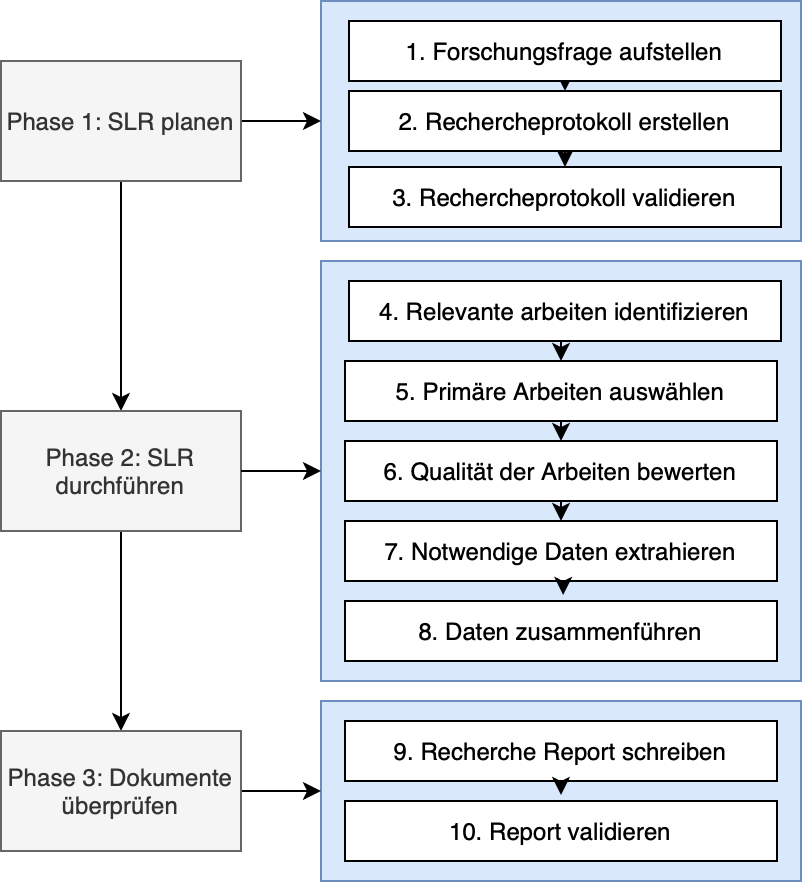
\includegraphics[width=0.8\textwidth]{graphics/slr_kitchenham_ablauf.png}
    \caption{Ablauf der systematischen Literaturrecherche nach Brereton et al. \cite{brereton2007lessons}}
    \label{fig:slr_kitchenham}
\end{figure}

\paragraph{Forschungsfrage}
Wie können Low-Code Entwicklungsansätze effektiv in die Konzeption und Entwicklung von Quantencomputing-Anwendungen 
integriert werden, unter besonderer Berücksichtigung von Model-Driven Engineering (MDE) und Open-Source-Prinzipien?

\paragraph{Suchstrategie und Datenbanken}
In den Suchmaschinen \textit{Google Scholar}, \textit{IEEE Xplore} und \textit{ACM Digital Library} 
wird gesucht. Die Auswahl der Suchbegriffe wird strategisch vorgenommen, um die Breite und Tiefe der beiden 
Hauptthemenbereiche abzudecken. 

Die Suchbegriffe der ersten Iteration sind
\begin{itemize}
    \item \textit{Low-Code Development} 
    \item \textit{Quantum Computing}
    \item \textit{Model-Driven Engineering}
    \item \textit{Open Source}
\end{itemize} 

Um die Schnittstellen zwischen Low-Code-Plattformen und Quantencomputing genauer zu untersuchen, 
wurden die Suchbegriffe in verschiedenen Kombinationen verwendet, wobei Boolesche Operatoren wie 
AND und OR zum Einsatz kommen, um die Suche zu verfeinern und zu spezifizieren.

Die Studien müssen frühestens ab dem Jahr 2014 veröffentlicht worden sein. Dies ist insbeondere in 
Hinsicht darauf wichtig, ob das entsprechendes Tool noch aktiv gewartet wird. 
Weiterhin ist die Aktualität der Studien wichtig, da sich die Technologien und Frameworks 
im Bereich Low-Code-Entwicklung und Quantencomputing schnell weiterentwickeln.

Es werden nur Studien in englischer oder deutscher Sprache berücksichtigt, die Peer-Review-Verfahren 
durchlaufen haben. Insbesondere als relevant werden Papers erachtet, die Low-Code-Plattformen 
in Open-Source Lizensierungen behandeln. Dies vereinfacht die Verwendbarkeit für 
die spätere pilothafte Umsetzung eines Low-Code Tools für Quantencomputing-Anwendungen.

Durch die Anwendung dieser 
methodischen und strukturierten Vorgehensweise wird eine solide Basis für die Erforschung 
und Analyse der Konzeption und Entwicklung von Low-Code-Frameworks für 
Quantencomputing-Anwendungen geschaffen.

\paragraph{ResearchRabbit}
In dieser Arbeit wird ResearchRabbit als ergänzendes Tool zur systematischen Literaturrecherche eingesetzt. 
ResearchRabbit ist ein Softwaretool, das entwickelt wurde, um Arbeiten aus Forschungsgebieten als Graph darzustellen 
und relevante Verbindungen zwischen wissenschaftlichen Publikationen auf Basis von Zitierungen und thematischen 
Ähnlichkeiten zu visualisieren.\cite{cole2023researchrabbit} Nutzer des Tools geben spezifische Suchbegriffe ein, woraufhin ResearchRabbit eine 
interaktive Map generiert. Diese Maps bieten eine visuelle Darstellung, die es ermöglicht, 
zentrale Arbeiten und bisher weniger beachtete Verbindungen schnell zu identifizieren.

Die Anwendung von ResearchRabbit in der systematischen Literaturrecherche bietet erhebliche Vorteile. Erstens 
steigert das Tool die Effizienz des Rechercheprozesses, indem es durch die Visualisierung von Forschungsnetzwerken 
relevante Studien schneller erkennbar macht, was den Zeitaufwand für das erste Screening reduziert. Zweitens 
erweitert ResearchRabbit die Möglichkeit, wichtige Arbeiten zu entdecken, die in traditionellen Datenbankensuchen 
möglicherweise übersehen werden würden. Dies geschieht insbesondere durch die Aufdeckung von Querverbindungen 
zwischen verschiedenen Forschungsgebieten. Darüber hinaus ermöglicht die Analyse von Netzwerkbeziehungen 
tiefere Einblicke in die Einflussnahme und den thematischen Kontext von Schlüsselpublikationen, was zu einem 
besseren Verständnis des Forschungsstandes beiträgt. Schließlich erlaubt das Tool, aktuelle Forschungsentwicklungen 
zu verfolgen und die Literaturrecherche regelmäßig mit neuen relevanten Publikationen zu aktualisieren.

Die Entscheidung, ResearchRabbit einzusetzen, basiert auf der Notwendigkeit, eine umfangreiche und 
dynamische Forschungslandschaft effektiv zu navigieren. In sich schnell weiterentwickelnden und interdisziplinären 
Feldern wie Low-Code Development und Quantum Computing bietet ResearchRabbit einen signifikanten Mehrwert, 
indem es komplexe Informationsstrukturen zugänglich und handhabbar macht. Durch die Integration dieses Tools 
in die systematische Literaturrecherche wird nicht nur die Effizienz des Prozesses verbessert, sondern auch 
die Qualität und Tiefe der Forschungsergebnisse erhöht.

\section{Durchführung der Literaturrecherche}
Basierend auf den im vorherigen Abschnitt festgelegten Kriterien wird die systematische Literaturrecherche (SLR) 
durchgeführt. Im Folgenden werden die einzelnen Schritte der Recherche detailliert dokumentiert und die Ergebnisse 
visualisiert. Dies umfasst die spezifischen Suchanfragen in den ausgewählten wissenschaftlichen Datenbanken, die 
angewandten Suchlimits sowie die quantitativen Ergebnisse der Suchvorgänge. Durch diese detaillierte Dokumentation 
wird die Nachvollziehbarkeit und Reproduzierbarkeit der Forschung sichergestellt, während die quantitativen 
Ergebnisse eine fundierte Basis für die weitere Analyse bieten.

\paragraph{Explorative Suche}
Die explorative Suche dient dazu, einen ersten Überblick über die verfügbare Literatur zu gewinnen und 
die Relevanz der Forschungsfrage zu überprüfen. Dabei werden die Suchbegriffe in den ausgewählten 
Datenbanken eingegeben und potenziell relevante Ergebnisse festgehalten. Dieser Schritt ermöglicht es, 
die Breite und Tiefe des Forschungsfeldes zu erfassen und die Suche gegebenenfalls zu verfeinern. 
Die Ergebnisse der explorativen Suche dienen auch als Ausgangspunkt für die systematische Literaturrecherche. 
Eine erste Anfrage in Google Scholar mit \textit{intitle:"low-code" tools platforms comparison overview} liefert 489 
Ergebnisse. Diese werden explorativ gesichtet und auf Relevanz geprüft. Insgesamt wurden initial 4 Publikationen 
als relevant identifiziert. Zwei davon sind insbesondere relevant, da sie einen Vergleich verschiedener 
Low-Code-Plattformen und deren Charakteristika ziehen. 

Durch Hinweise auf MDE und LCD Lösungen einmal aus dem Quantencomputing und einmal aus dem Open Source Bereich werden 
weiterhin zwei Publikationen hinzugenommen. Diese sind zum eine Publikation über \textit{Classiq} \cite{minerbi2022quantum}, zum anderen 
eine Publikation über \textit{BESSER} \cite{alfonso2024building}. 

% ggf related work ⬇️
Classiq ist ein Framework zur Entwicklung von Quantencomputeralgorithmen, das darauf abzielt, die Komplexität der Programmierung 
auf Gatterniveau zu reduzieren und die Zugänglichkeit für Entwickler zu verbessern. Es ermöglicht die Erstellung optimierter und 
hardwarebewusster Quantenschaltkreise aus hochabstrakten funktionalen Modellen. Diese Plattform automatisiert den Prozess der 
Quantenalgorithmuserstellung, indem sie Nutzern erlaubt, sich auf die funktionalen Anforderungen zu konzentrieren, während die 
Plattform die Details der Schaltkreisimplementierung übernimmt.

Ein Hauptvorteil von Classiq ist die Möglichkeit, Quantenalgorithmen visuell zu entwerfen und automatisch die besten Implementierungsoptionen 
zu ermitteln, die den Systemanforderungen und Hardwarebeschränkungen entsprechen. Dies reduziert den Aufwand für die manuelle Codierung und 
Optimierung erheblich. Classiq unterstützt zudem die Integration domänenspezifischer Expertise, was die Entwicklung spezialisierter 
Quantenlösungen in Bereichen wie Finanzwesen, Chemie und Cybersicherheit erleichtert.

Zusätzlich bietet Classiq Werkzeuge wie Schaltkreisvisualisierungen und Hardwarevergleichstabellen, die Entwicklern helfen, die 
besten Hardwareoptionen für ihre Algorithmen zu identifizieren und zu testen, ohne tiefgehende Hardwarekenntnisse zu benötigen. 
Diese Features tragen dazu bei, Quantencomputing für eine breitere Nutzerbasis zugänglich zu machen, von 
Quantenexperten bis hin zu Domänenexperten, die keine tiefen Kenntnisse in Quantenphysik besitzen.

Durch diese Funktionen unterstützt Classiq die Innovation und Kollaboration im Bereich Quantencomputing und ebnet den 
Weg für die Entwicklung fortschrittlicher Quantenanwendungen \cite{minerbi2022quantum}. 

Das BESSER-Framework ist eine Open-Source-Low-Code-Plattform. Die Plattform enthält verschiedene Code-Generatoren, die automatisch Code 
für unterschiedliche Programmiersprachen und Frameworks generieren können. 

Ein Merkmal von BESSER ist seine Erweiterbarkeit und Anpassungsfähigkeit. Die Plattform ist so konzipiert, dass sowohl die 
Spezifikationsmethoden als auch die Code-Generatoren von der Community erweitert und angepasst werden können. Dies fördert 
nicht nur die Innovation innerhalb der Entwicklergemeinschaft, sondern ermöglicht es auch, spezifische Anforderungen und 
Präferenzen der Nutzer zu berücksichtigen. Da BESSER eine Open-Source-Plattform ist, können Nutzer die Plattform frei 
modifizieren und erweitern, was die Gefahr von Vendor-Lock-ins minimiert und die Flexibilität erhöht.

Darüber hinaus adressiert BESSER die wachsende Komplexität moderner Softwaresysteme, indem es Low-Code-Entwicklungsansätze mit 
fortschrittlichen Modellierungs- und Generierungstechniken kombiniert. Dies macht es zu einem geeigneten Werkzeug für die Entwicklung 
komplexer, intelligenter Softwarelösungen, die auf die Bedürfnisse einer breiten Nutzerbasis 
zugeschnitten sind, von technischen Experten bis hin zu Geschäftsanwendern \cite{alfonso2024building}.
% ggf related work ⬆️

\paragraph{Protokollbasierte Suche}
Im Schritt der protokollbasierten Suche werden die vorgestellten Suchbegriffe und Kriterien für die systematische Literaturrecherche 
angewandt. 
In der Grafik \ref{fig:search_process} ist der Ablauf der Suche nach Publikationen innerhalb der 
systematischen Literaturrecherche dargestellt. Insbesondere wird hier nochmal erwähnt, dass beim Schritt des 
Snowballings das Tool ResearchRabbit eingesetzt wird, um die Suche zu unterstützen. 

% include graphics/ablauf_der_suche.png
\begin{figure}[h!]
    \centering
    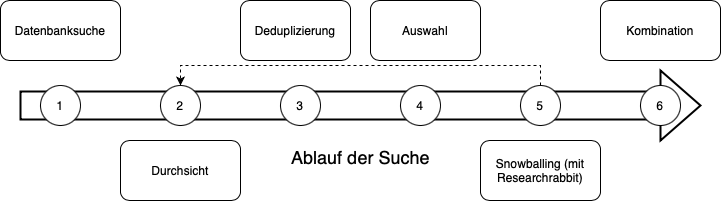
\includegraphics[width=1\textwidth]{graphics/ablauf_der_suche.png}
    \caption{Ablauf der systematischen Literaturrecherche}
    \label{fig:search_process}
\end{figure}

Um einen ersten Überblick über die Publikationen zu gewinnen wird initial die folgende Suchanfrage in den Datenbanken verwendet:

\begin{quote}
    Suchanfrage 1 (Stand: 12.07.2024):

    (''Low-Code Development'' OR ''Quantum Computing'' OR ''Model-Driven Engineering'' OR ''Open Source'')

    Erscheinungsdatum der Publikationen: 2014 - 2024
\end{quote}

\begin{table}[h!]
    \centering
    \caption{Anzahl der Suchergebnisse für Suchanfrage 1}
    \label{tab:search_1_results}
    \begin{tabular}{|l|c|}
    \hline
    \textbf{Datenbank} & \textbf{Anzahl der Ergebnisse} \\ \hline
    Google Scholar & 17.800 \\ \hline
    IEEE Xplore & 62.421 \\ \hline
    ACM Digital Library & 79.035 \\ \hline
    \end{tabular}
\end{table}
    
Diese Suchanfrage lieferte die in \ref{tab:search_1_results} dargestellten Ergebnisse. Dies 
zeigt die große Bandbreite und Relevanz der Themenfelder. 
Um hier einen Überblick zu gewinnen, wie die Verteilung der Publikationen zu den jeweiligen Konzepten ausfällt, 
wird eine Analyse der Anzahl der Publikationen pro Jahr, und Konzept, also MDE oder Low-Code vorgenommen.

Deren Ergebnisse sind in den folgenden Grafiken dargestellt:

\begin{figure}[h!]
    \centering
    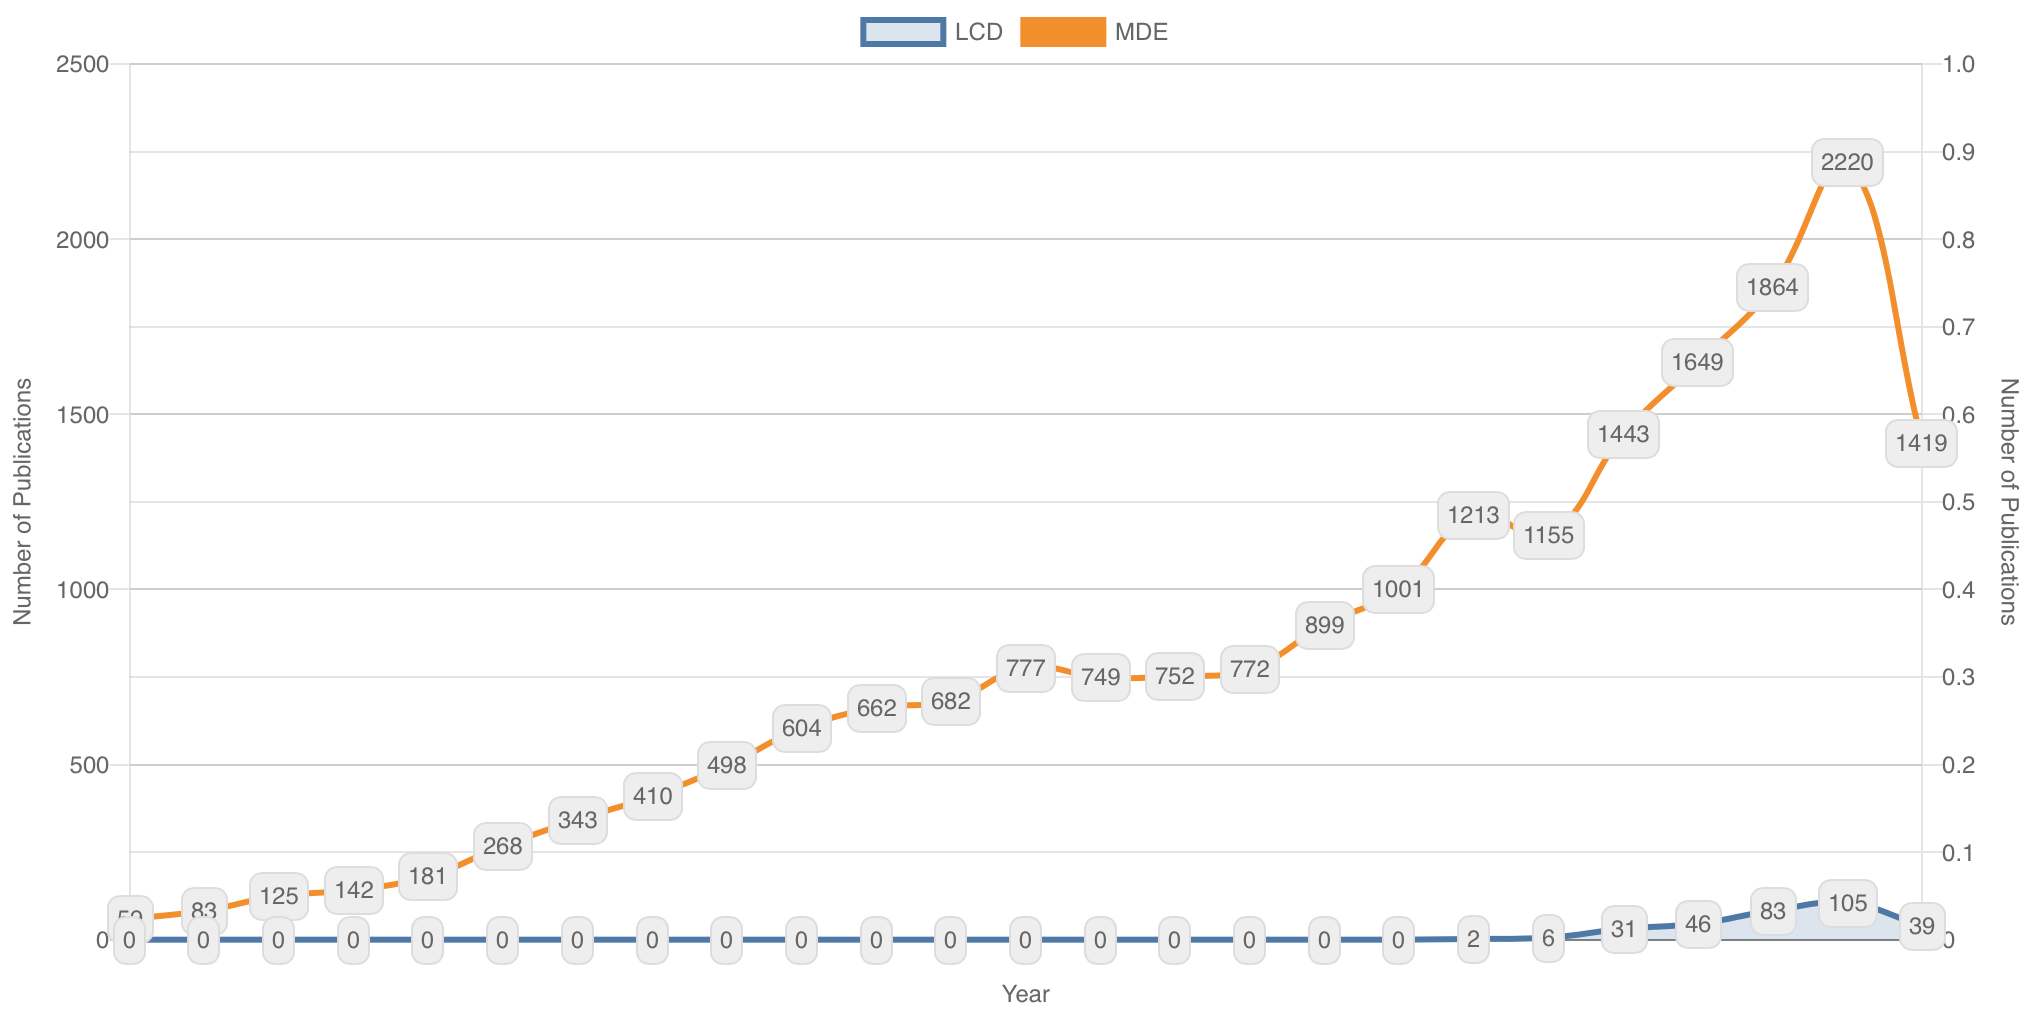
\includegraphics[width=1\textwidth]{graphics/lcd_and_mde_publications_over_years.png}
    \caption{Anzahl der Publikationen zu MDE und LCD pro Jahr}
    \label{fig:publications_mde_and_lcd_per_year}
\end{figure}

\begin{figure}[h!]
    \centering
    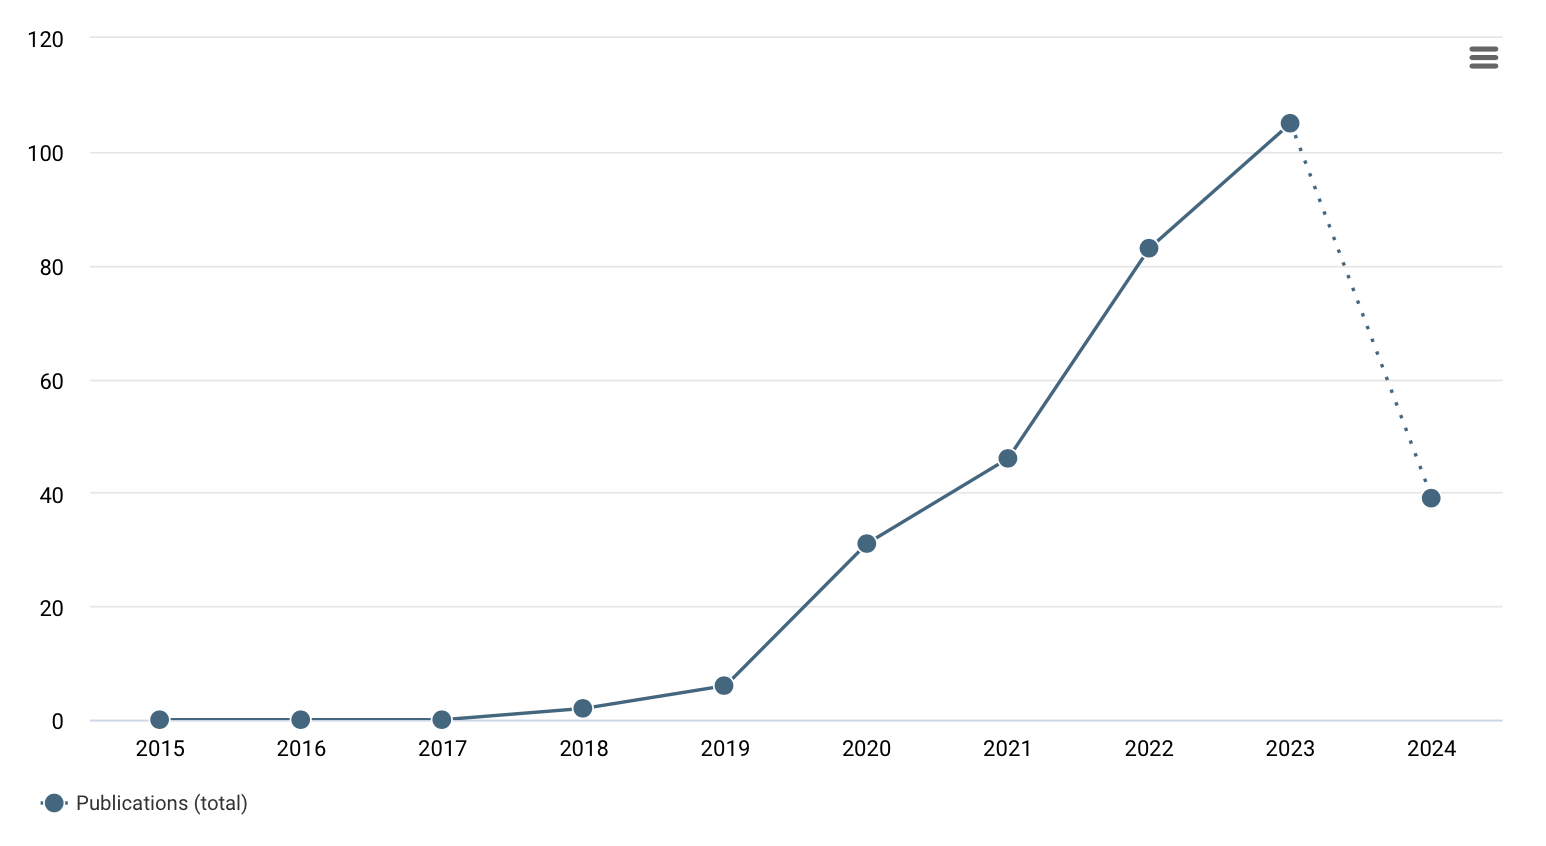
\includegraphics[width=1\textwidth]{graphics/lcd_publications_over_years.png}
    \caption{Anzahl der Publikationen LCD pro Jahr}
    \label{fig:publications_lcd_per_year}
\end{figure}

\begin{figure}[h!]
    \centering
    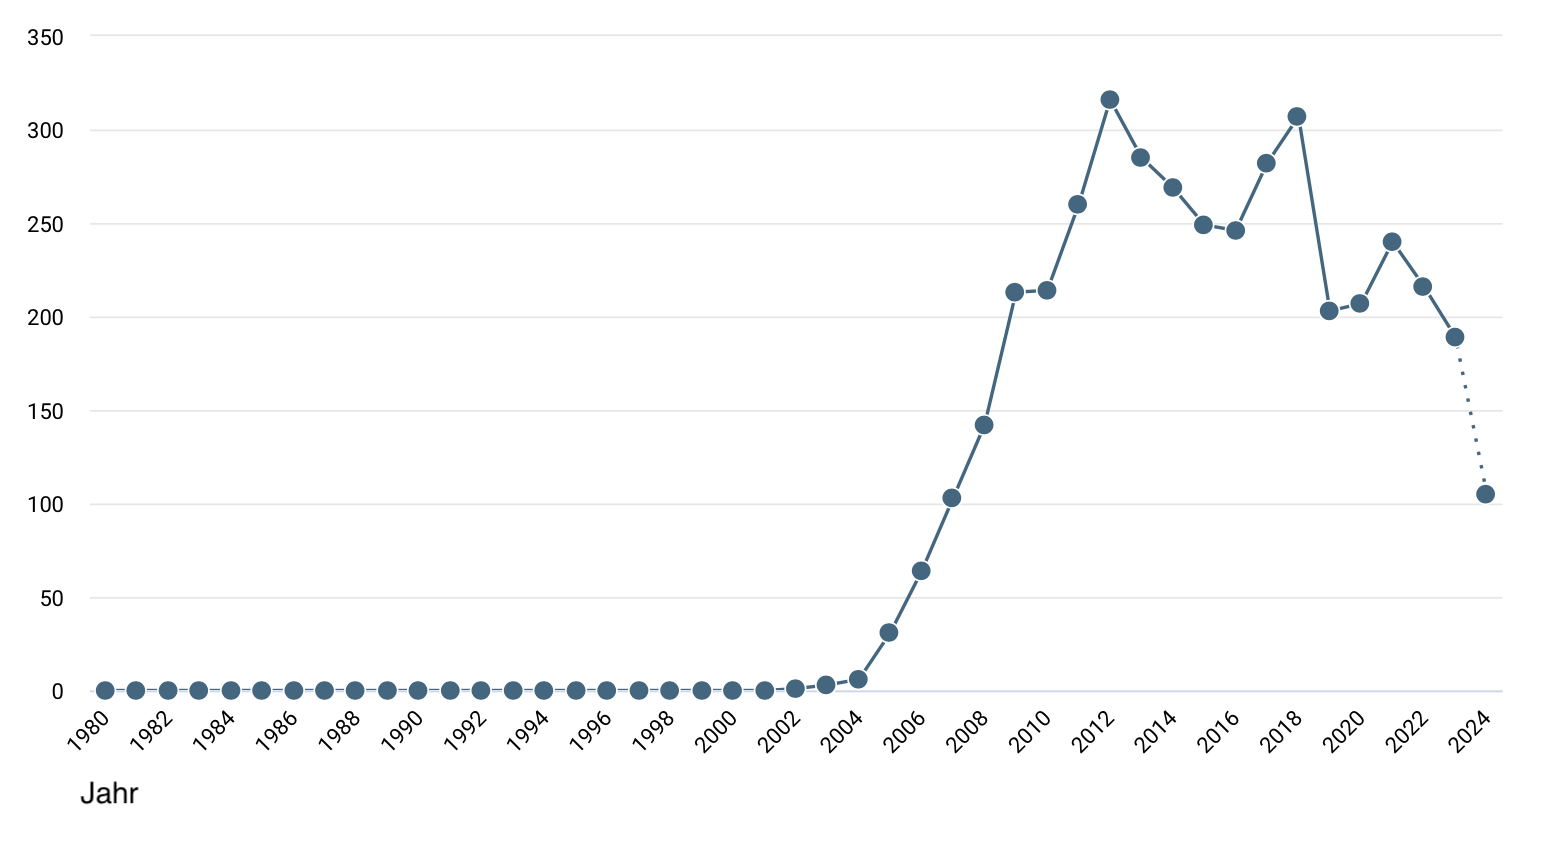
\includegraphics[width=1\textwidth]{graphics/mde_publications_over_years.png}
    \caption{Anzahl der Publikationen zu MDE pro Jahr}
    \label{fig:publications_mde_per_year}
\end{figure}

Es fällt auf, dass die Anzahl der Publikationen zu Low-Code-Entwicklung erstens insgesamt deutlich niedriger ausfällt 
als die Anzahl der Publikationen zu Model-Driven Engineering. Zweitens ist bezüglich des Erscheinungsjahres festzustellen 
das in Publikation Low-Code-Entwicklung ein deutlich jüngeres Forschungsthema ist.

Da die Anzahl der Ergebnisse zu groß ist um effektiv bearbeitet zu werden, wird die Suche 
weiter verfeinert. Weiterhin fällt beim ersten Screening auf, dass viele Ergebnisse nicht die 
gewünschte Schnittmenge aus Low-Code-Entwicklung und Quantencomputing abdecken, sondern 
nur eines der beiden Themenfelder behandeln. Um also die Relevanz der Ergebnisse zu erhöhen, 
werden spezifischere Suchanfragen formuliert. 

In einer zweiten Iteration der Suche wurde daher die folgende Suchanfrage verwendet:

\begin{quote}
    Suchanfrage 2 (Stand: 14.07.2024):

    (''Low Code Platform'' OR ''Low Code Development'' OR ''Low-Code Development'' OR ''Model-Driven Engineering'') AND (''Quantum Computing'')

    Erscheinungsdatum der Publikationen: 2014 - 2024
\end{quote}

\begin{table}[h!]
    \centering
    \caption{Anzahl der Suchergebnisse für Suchanfrage 2}
    \label{tab:search_2_results}
    \begin{tabular}{|l|c|}
    \hline
    \textbf{Datenbank} & \textbf{Anzahl der Ergebnisse} \\ \hline
    Google Scholar & 176 \\ \hline
    IEEE Xplore & 3 \\ \hline
    ACM Digital Library & 30 \\ \hline
    \end{tabular}
\end{table}

Die Ergebnisse der zweiten Suchanfrage sind in Tabelle \ref{tab:search_2_results} dargestellt. Bzgl. der Erscheinungsjahre fällt auf, dass in 
IEEE Xplore die drei Publikationen zwischen 2021 und 2023 erschienen. in der ACM Digital Library sind die Publikationen zwischen 2021 und 2024 erschienen. 
Lediglich die Google Scholar Suche ergab Publikationen, die bis ins Jahr 2014 als Untergrenze der gewünschten Filterung zurückreichen. 

Da die Anzahl der Ergebnisse nun sinnvoller ist, wird mit der Durchsicht der Titel und Abstracts fortgefahren. 
Begonnen wird mit den drei Ergebnissen aus IEEE Xplore. Durchsicht der Abstracts ergibt, dass die Publikationen 
alle drei relevant sind, da sie sich inhaltlich in der Schnittmenge aus MDE und Quantencomputing befinden. 
Um für die Datenbank IEEE Xplore den Schritt der Auswahl vorwegzugreifen, werden die drei Publikationen 
direkt in die engere Auswahl übernommen. 

Als nächsten werden die Ergebnisse der ACM Digital Library ebenfalls durchgesehen. Dabei werden beim Schritt der Auswahl notwendigerweise die 
Ergebnisse der ACM Digital Library gezielt gefiltert, um die Relevanz und Qualität der eingeschlossenen Studien sicherzustellen. 
Proceedings wurden dabei bewusst nicht in die Auswahl einbezogen. Der Grund dafür ist, dass Proceedings häufig eine 
Vielzahl von Kurzbeiträgen enthalten, die nicht denselben rigorosen Peer-Review-Prozess durchlaufen wie Journal-Artikel 
und oft eine geringere wissenschaftliche Tiefe aufweisen. Dies kann die Validität und Verlässlichkeit der 
Forschungsergebnisse beeinträchtigen. Zudem sind Proceedings meist vorläufige Ergebnisse, die 
später in detaillierteren Journal-Artikeln veröffentlicht werden. Von den initialen 30 Ergebnissen 
in der ACM Digital Library erfüllten lediglich 4 die AuswahlkriterienDurch diese Vorgehensweise wurde 
sichergestellt, dass nur qualitativ hochwertige und relevante Studien in die Analyse einbezogen wurden.

Weiterhin wurden Publikationen ausgeschlossen, deren Titel oder Abstract darauf schließen ließen, dass sie thematisch 
nicht relevant sind. Dieser Ausschluss erfolgte, um die Fokussierung auf Studien zu gewährleisten, die direkt mit 
Low-Code-Entwicklungsansätzen in Quantencomputing-Anwendungen verbunden sind. Diese strenge Selektion ist entscheidend, um 
sicherzustellen, dass die verbleibenden Studien tatsächlich die Forschungsfrage adressieren und qualitative Erkenntnisse liefern können. 

Durchsicht der 176 Ergebnisse aus Google Scholar ergab, dass 20 Publikationen die Kriterien für die engere Auswahl erfüllen. 

Für den Schritt der Deduplizierung wurden die Ergebnisse aus den drei Datenbanken zusammengeführt. 
So ergeben sich ohne Duplikate insgesamt 25 Publikationen, die für die weitere Analyse in Betracht gezogen werden. 

Bevor durch Snowballing weitere möglicherweise relevante Publikationen gesucht werden und die Volltexte der Publikationen analysiert werden, 
wird eine dritte Suchanfrage formuliert. Diese zielt darauf ab, durch eine noch feinere Fomulierung der Anfrage weitere bisher nicht gefundene 
Ergebnisse zu identifizieren. 

\begin{quote}
    Suchanfrage 3 (Stand: 16.07.2024):

    (intitle:''low-code'' quantum computing)

    Erscheinungsdatum der Publikationen: 2014 - 2024
\end{quote}

Hierfür ergibt sich die in Tabelle \ref{tab:search_3_results} dargestellte Anzahl an Ergebnissen. 

\begin{table}[h!]
    \centering
    \caption{Anzahl der Suchergebnisse für Suchanfrage 3}
    \label{tab:search_3_results}
    \begin{tabular}{|l|c|}
    \hline
    \textbf{Datenbank} & \textbf{Anzahl der Ergebnisse} \\ \hline
    Google Scholar & 26 \\ \hline
    IEEE Xplore & 1 \\ \hline
    ACM Digital Library & 8 \\ \hline
    \end{tabular}
\end{table}

Erneut ist die Anzahl an Suchergebnissen geringer geworden. Durchsicht der neuen Ergebnisse ergibt, dass zwar aus Google Scholar 
keine weiteren Publikationen in die engere Auswahl übernommen werden, jedoch aus der ACM Digital Library 7 sowie aus IEEE Xplore 1 Publikation. 
Insgesamt ergibt sich somit eine Anzahl von 33 unterschiedlichen Publikationen, die für die weitere Analyse in Betracht gezogen werden. 

Mit den nun identifizierten Publikationen wird der Schritt des Snowballings durchgeführt. Hierbei wird ResearchRabbit eingesetzt, um 
weitere Publikationen zu identifizieren, die inhaltlich mit den bereits identifizierten Publikationen in Verbindung stehen und somit 
potenziell relevant sind. Das Tool zeigt dabei die Verbindungen zwischen den Publikationen an und ermöglicht es, die Netzwerke 
zu älteren und neueren Publikationen zu visualisieren. Es ergeben sich 21 ältere Publikationen, die mit den bereits identifizierten 33 
Publikationen in Verbindung stehen. Dazu kommen 6 neuere die auf die bereits identifizierten Publikationen verweisen. 

Für diese wird nun ebenfalls der Titel und Abstract durchgesehen, um zu entscheiden, ob sie in die engere Auswahl übernommen werden. 
Insgesamt lassen sich so 13 weitere Publikationen identifizieren, die für die weitere Analyse in Betracht gezogen werden. 

Um sicherzustellen, dass alle identifizierten Publikationen relevant sind für die thematische Schnittmenge aus Low-Code Development bzw. 
MDE und Quantencomputing, werden die Abstracts aller Publikationen analysiert. Dabei wird geprüft, ob die Publikationen die 
Forschungsfrage adressieren und qualitative Erkenntnisse liefern können. 

\section{Ergebnisse}
Insgesamt ergeben sich somit aus der explorativen und protokollbaiserten Suche 41 Publikationen, die für die weitere Analyse 
in Betracht gezogen werden. 

Die Verteilung der Publikationen auf die Jahre ist in Grafik \ref{fig:publications_per_year} dargestellt.

\begin{figure}[h!]
    \centering
    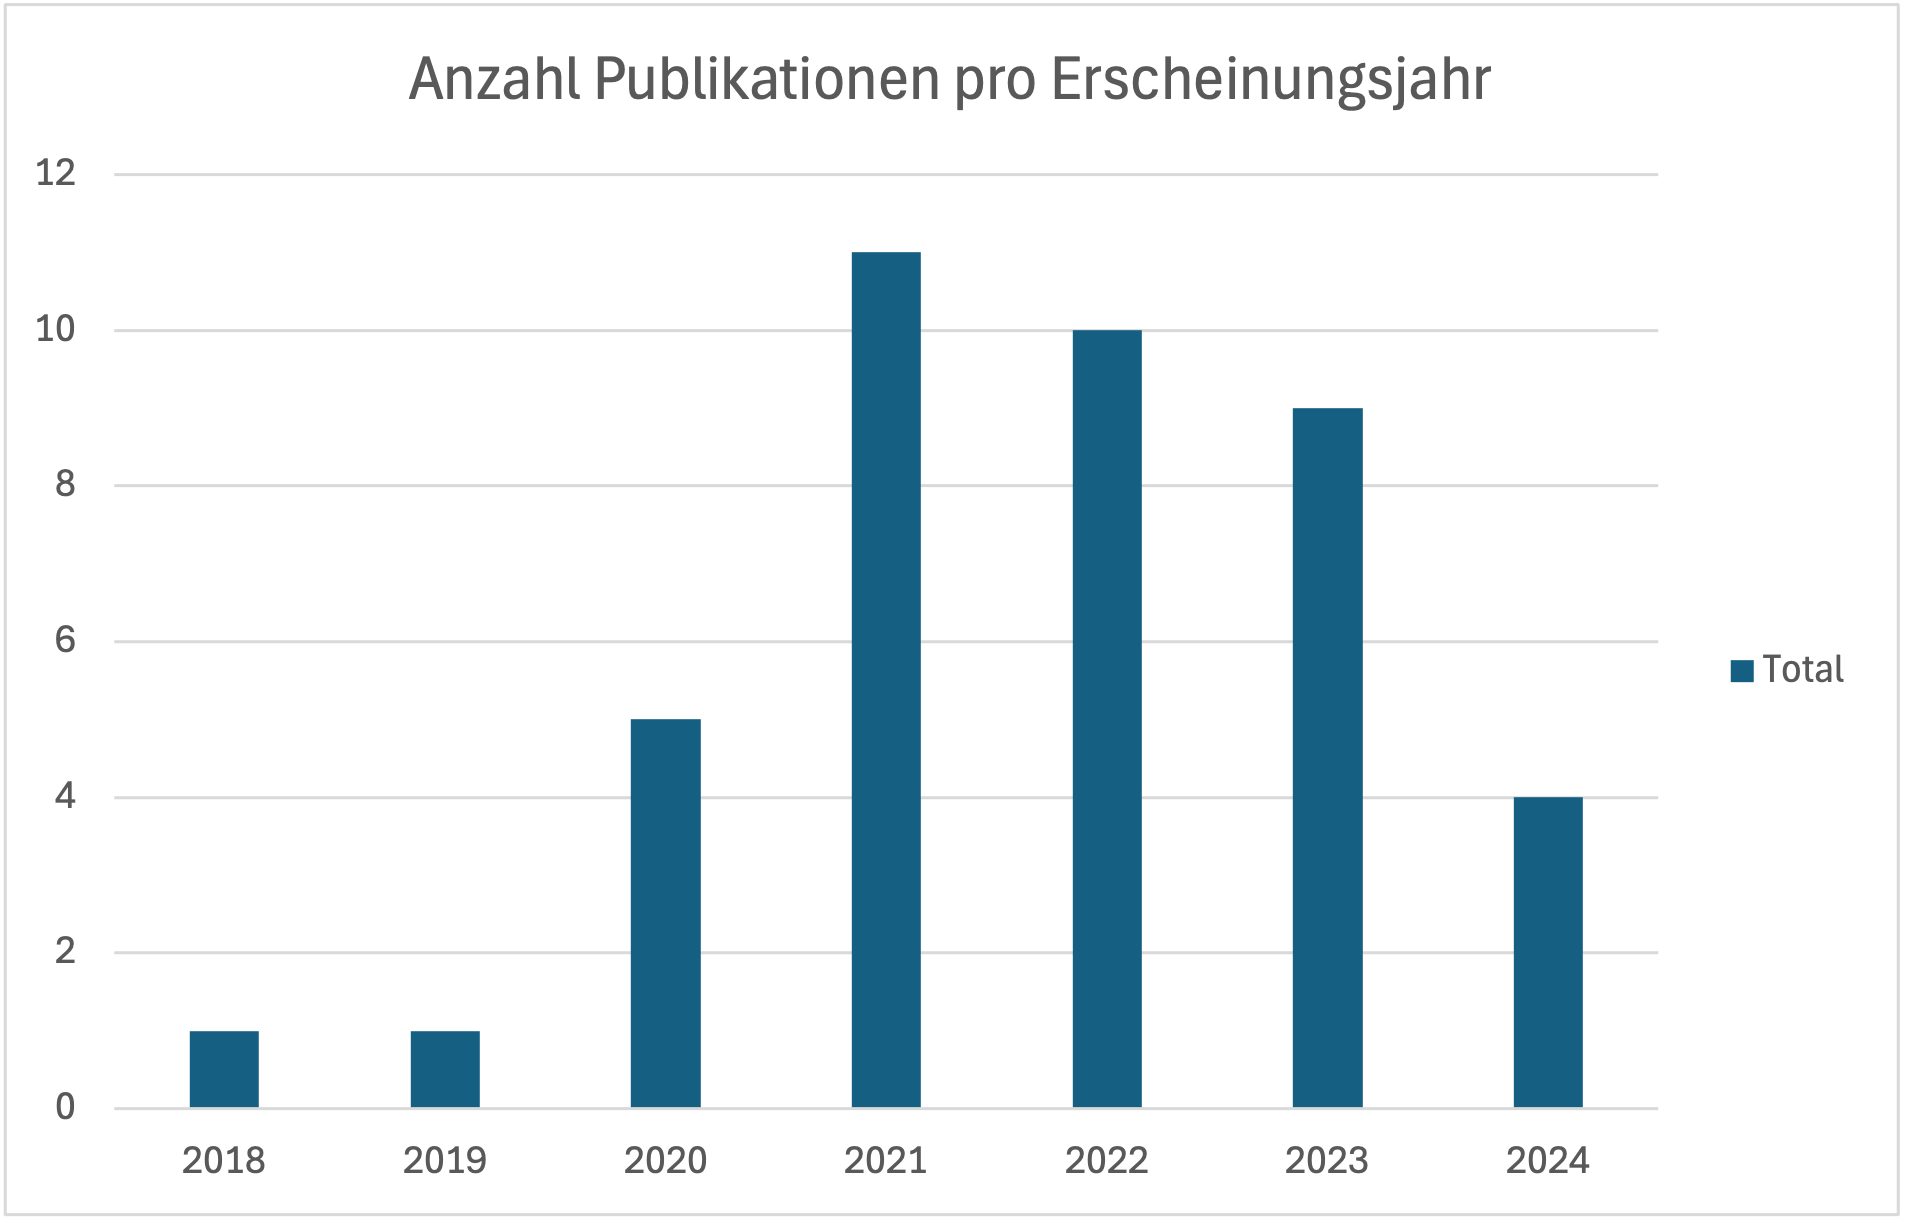
\includegraphics[width=0.8\textwidth]{graphics/anzahl_pubs_jahr.png}
    \caption{Anzahl der Publikationen pro Jahr}
    \label{fig:publications_per_year}
\end{figure}

Die Kategorisierung nach Themenbereichen ist in der Grafik \ref{fig:publications_per_topic} dargestellt.

\begin{figure}[h!]
    \centering
    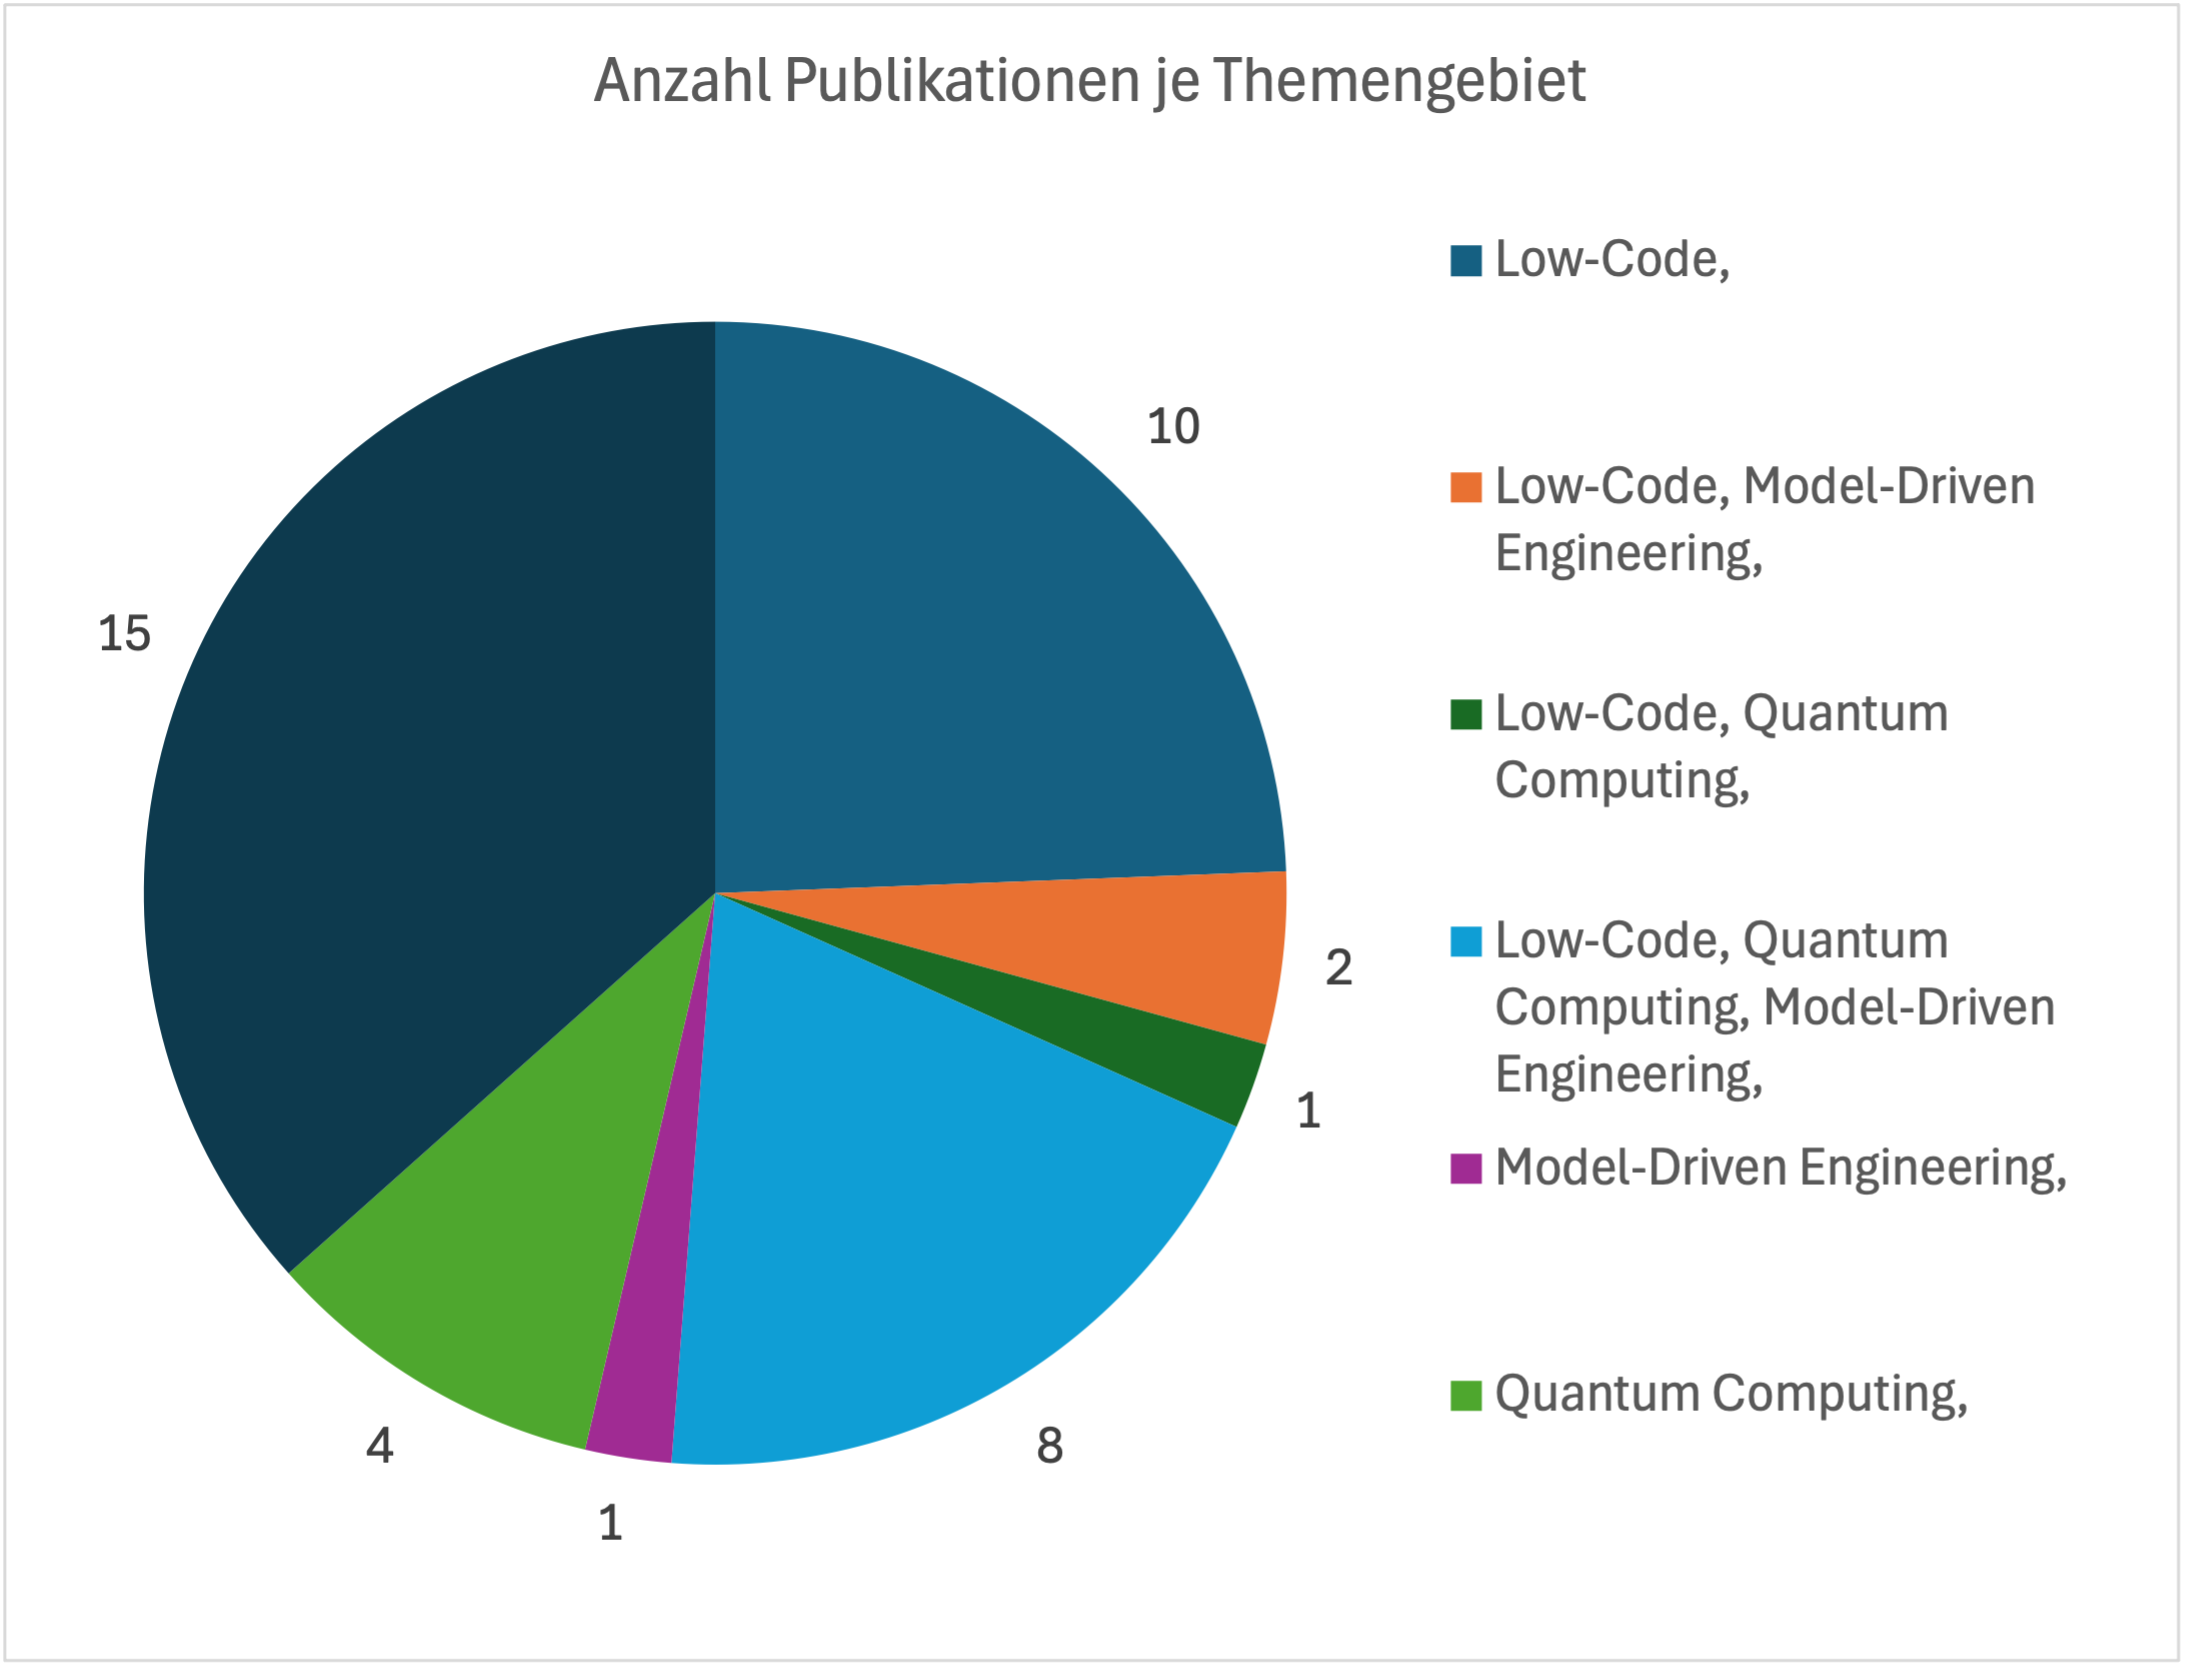
\includegraphics[width=0.8\textwidth]{graphics/anzahl_themen_pubs.png}
    \caption{Anzahl der Publikationen pro Themenbereich}
    \label{fig:publications_per_topic}
\end{figure}

%  ggf kommt hier auch das ganze quantitave erklärzeugs was bisher im abschnitt davor mit drin ist, vllt kann mans au mergen

\section{Synthese und Bewertung der Ergebnisse}
Die Synthese und Bewertung der Ergebnisse erfolgt in mehreren Schritten, um die identifizierten Studien zu analysieren, 
zu interpretieren und zu bewerten. Dabei werden die Hauptbefunde zusammengefasst, die Erkenntnisse integriert und 
Forschungslücken identifiziert. 

Vor dem Hintergrund der gestellten Forschungsfrage werden Kriterien aufgestellt, anhand derer die Publikationen 
bewertet werden. In Tabelle \ref{tab:evaluation_criteria} sind die Kriterien dargestellt, die für die Forschungsfrage 
herangezogen werden. 

\begin{table}[h!]
    \centering
    \caption{Kriterien zur Bewertung der Publikationen}
    \label{tab:evaluation_criteria}
    \begin{tabular}{|p{5cm}|p{9cm}|}
    \hline
    \textbf{Kriterium} & \textbf{Beschreibung} \\ \hline
    Low-Code Tools & Welche Low-Code Tools, Plattformen oder Konzepte werden erwähnt? \\ \hline
    Quantencomputing & Werden Möglichkeiten der Anwendung im Quantencomputing erwähnt, und falls ja, welche? \\ \hline
    Aktualität & Wie aktuell sind die in der Publikation behandelten Konzepte und Tools? \\ \hline
    Open-Source & Sind die erwähnten Ansätze frei zugänglich oder kommerziell? \\ \hline
    \end{tabular}
\end{table}

\paragraph{Supporting the understanding and comparison of low-code development platforms}

Das Paper von Apurvanand Sahay et al. (2020) untersucht verschiedene Low-Code-Entwicklungsplattformen und vergleicht deren 
Eigenschaften und Fähigkeiten. Zu den untersuchten Plattformen gehören OutSystems, Mendix, Appian, PowerApps und Salesforce. 
Diese Plattformen werden hinsichtlich ihrer Benutzerfreundlichkeit, Anpassungsfähigkeit und Integration in bestehende Systeme analysiert.

Das Paper diskutiert ausführlich die folgenden Low-Code-Entwicklungsplattformen: OutSystems, Mendix, Appian, PowerApps und Salesforce. 
Diese Tools werden hinsichtlich ihrer Funktionen und Einsatzmöglichkeiten im klassischen Softwareentwicklungsprozess untersucht.
Möglichkeiten der Anwendung im Quantencomputing werden in diesem Paper nicht erwähnt. Der Fokus liegt ausschließlich auf klassischen 
Low-Code-Plattformen und deren Vergleich.
Das Paper wurde im Jahr 2020 veröffentlicht und behandelt die zu diesem Zeitpunkt aktuellen Konzepte und Tools. Die behandelten 
Plattformen und deren Funktionen spiegeln den Stand der Technik zur Zeit der Veröffentlichung wider.
Die im Paper erwähnten Low-Code-Plattformen sind kommerzielle Produkte. Es wird nicht auf Open-Source-Alternativen 
eingegangen, sondern auf etablierte, proprietäre Lösungen.

\paragraph{In Search of the Essence of Low-Code: An Exploratory Study of Seven Development Platforms}

Das Paper von Alexander C. Bock (2021) bietet eine tiefgehende Analyse von sieben verschiedenen Low-Code-Entwicklungsplattformen. 
Es untersucht die Kernmerkmale dieser Plattformen und beleuchtet deren Einsatzmöglichkeiten sowie Einschränkungen. Die analysierten 
Plattformen umfassen Betty Blocks, GeneXus, Quick Base, OutSystems, Mendix, PowerApps und Salesforce.

Es werden die Kernmerkmale, Einsatzmöglichkeiten und Einschränkungen dieser Plattformen detailliert beschrieben. 
Möglichkeiten der Anwendung im Quantencomputing werden in diesem Paper ebenfalls nicht behandelt. 
Der Fokus liegt auf der Analyse und dem Vergleich der Plattformen im Kontext klassischer Softwareentwicklungsprozesse. 
Die Studie wurde im Jahr 2021 durchgeführt und behandelt aktuelle Konzepte und Tools zur Zeit der Veröffentlichung. 
Die im Paper untersuchten Low-Code-Plattformen sind sowohl kommerzielle als auch proprietäre Lösungen, 
wobei Open-Source-Alternativen nicht im Fokus stehen.

\paragraph{What about the usability in low-code platforms? A systematic literature review}

Das Paper von Daniel Pinho und Vasco Amaral (2022) bietet eine systematische Literaturübersicht zur Benutzerfreundlichkeit von 
Low-Code-Plattformen. Es untersucht die wichtigsten Kriterien und Herausforderungen im Zusammenhang mit der Usability 
dieser Plattformen und analysiert eine Vielzahl von bestehenden Studien, um ein umfassendes Bild der aktuellen Forschungslage zu zeichnen.

Das Paper identifiziert und bewertet mehrere Low-Code-Entwicklungsplattformen, allerdings werden spezifische Plattformen 
und Tools nicht namentlich genannt. Der Schwerpunkt liegt auf der Analyse von Benutzerfreundlichkeit und den damit 
verbundenen Herausforderungen, wie zum Beispiel der Lernkurve für neue Nutzer und der Anpassungsfähigkeit der 
Plattformen an unterschiedliche Nutzerbedürfnisse. 
Möglichkeiten der Anwendung im Quantencomputing werden in diesem Paper nicht diskutiert. 
Die Untersuchung konzentriert sich ausschließlich auf die Benutzerfreundlichkeit von Low-Code-Plattformen. 
Das Paper wurde 2022 veröffentlicht und bezieht sich auf aktuelle Konzepte und Entwicklungen in der Low-Code-Entwicklung. 
Es wird nicht explizit zwischen kommerziellen und Open-Source-Lösungen unterschieden, 
sondern allgemein die Usability von Low-Code-Plattformen untersucht.

\paragraph{Low-Code Development Platforms - A Literature Review}

Das Paper von Niculin Prinz und Melanie Huber (2021) bietet einen umfassenden Literaturüberblick über Low-Code-Entwicklungsplattformen. 
Es untersucht die verschiedenen Aspekte und Eigenschaften dieser Plattformen, einschließlich ihrer Vorteile, Herausforderungen 
und Anwendungsbereiche. Die Autoren analysieren eine breite Palette von Studien, um die wesentlichen Merkmale und Trends 
in der Low-Code-Entwicklung zu identifizieren.

Das Paper identifiziert und bewertet mehrere Low-Code-Entwicklungsplattformen, darunter auch spezifische Plattformen wie 
OutSystems, Mendix und Appian. Es werden die Vorteile dieser Plattformen, wie z.B. die erhöhte Entwicklungsgeschwindigkeit und 
die Reduzierung von Kosten, sowie die Herausforderungen, wie die Abhängigkeit von proprietären Lösungen und die begrenzte 
Anpassungsfähigkeit, diskutiert. Möglichkeiten der Anwendung im Quantencomputing werden in diesem Paper nicht behandelt. 
Der Fokus liegt auf der allgemeinen Analyse und Bewertung von Low-Code-Plattformen im Kontext 
klassischer Softwareentwicklungsprozesse. Das Paper wurde 2021 veröffentlicht und 
bezieht sich auf aktuelle Konzepte und Entwicklungen in der Low-Code-Entwicklung. Es wird sowohl auf kommerzielle als 
auch auf Open-Source-Lösungen eingegangen, wobei ein Schwerpunkt auf der Bewertung der allgemeinen Marktsituation liegt.

\paragraph{AI for Low-Code for AI}

Das Paper von Nikitha Rao, Jason Tsay, Kiran Kate, Vincent Hellendoorn und Martin Hirzel (2024) untersucht den Einsatz 
von Künstlicher Intelligenz (KI) zur Verbesserung von Low-Code-Plattformen, die wiederum zur Entwicklung von KI-Anwendungen 
verwendet werden. Das Ziel des Papers ist es, die Synergien zwischen Low-Code-Entwicklung und KI zu beleuchten und zu 
zeigen, wie diese Technologien zusammenarbeiten können, um die Anwendungsentwicklung zu beschleunigen und zu vereinfachen.

Das Paper stellt verschiedene Low-Code-Plattformen vor, die speziell für die Entwicklung von KI-Anwendungen optimiert wurden, 
darunter Tools und Frameworks, die die Erstellung und Implementierung von KI-Modellen unterstützen. 
Es werden die Vorteile dieser Ansätze hervorgehoben, wie z.B. die Vereinfachung komplexer Entwicklungsprozesse, 
die Verbesserung der Zugänglichkeit für nicht-technische Nutzer und die Beschleunigung der Entwicklungszyklen. 
Möglichkeiten der Anwendung im Quantencomputing werden in diesem Paper nicht diskutiert. 
Der Fokus liegt auf der Integration von KI in Low-Code-Plattformen und deren Anwendung in der klassischen Softwareentwicklung. 
Das Paper wurde 2024 veröffentlicht und behandelt die neuesten Entwicklungen und Trends in diesem Bereich. 
Es wird sowohl auf kommerzielle als auch auf Open-Source-Lösungen eingegangen, wobei die 
Vorteile und Herausforderungen der Integration von KI in Low-Code-Entwicklungsplattformen analysiert werden.

\paragraph{Challenges \& Opportunities in Low-Code Testing}

Die Publikation von Faezeh Khorram, Jean-Marie Mottu und Gerson Sunyé (2020) untersucht die Herausforderungen und Chancen 
im Zusammenhang mit dem Testen von Low-Code-Anwendungen. Sie bietet eine detaillierte Analyse der spezifischen Anforderungen 
und Hindernisse, die bei der Qualitätssicherung von Anwendungen auftreten, die mit Low-Code-Plattformen entwickelt wurden.

In der Publikation werden mehrere Low-Code-Entwicklungsplattformen untersucht, darunter kommerzielle Tools wie OutSystems, 
Mendix und Appian. Ein besonderer Fokus liegt auf den neuen Konzepten und Charakteristika, die Low-Code-Plattformen in 
den Entwicklungsprozess einführen und die damit verbundenen Auswirkungen auf Teststrategien. Möglichkeiten der Anwendung 
im Quantencomputing werden in dieser Publikation nicht behandelt. Der Schwerpunkt liegt auf den Herausforderungen 
des Low-Code-Testings, einschließlich der Rolle von "Citizen Developers" im Testprozess, der Notwendigkeit hochgradiger 
Testautomatisierung und der speziellen Anforderungen an Cloud-Testing. Die Publikation wurde 2020 veröffentlicht und 
behandelt aktuelle Entwicklungen und Konzepte im Bereich des Low-Code-Testings. Es wird sowohl auf kommerzielle als 
auch auf Open-Source-Ansätze eingegangen, wobei die verschiedenen Herausforderungen und Chancen im Zusammenhang mit 
dem Testen von Low-Code-Anwendungen detailliert analysiert werden.

\paragraph{Quantumoonlight: A Low-Code Platform to Experiment with Quantum Machine Learning}

Die Publikation von Francesco Amato und Matteo Cicalese (2023) stellt die Low-Code-Plattform Quantumoonlight vor, 
die speziell für Experimente mit Quantum Machine Learning (QML) entwickelt wurde. Diese Plattform zielt darauf ab, 
die Komplexität der Entwicklung von QML-Anwendungen zu reduzieren und sowohl Forschern als auch Entwicklern eine 
benutzerfreundliche Umgebung zu bieten, in der sie ihre Algorithmen testen und validieren können.

Quantumoonlight bietet eine Reihe von Tools und Funktionen, die es ermöglichen, Quantenalgorithmen zu modellieren und in 
einer intuitiven, visuellen Umgebung zu implementieren. Die Plattform erleichtert den Einstieg in das Quantencomputing, 
indem sie die technischen Hürden senkt und es Nutzern ermöglicht, sich auf die Entwicklung und Optimierung von Algorithmen zu konzentrieren. 

Die Publikation hebt hervor, dass Quantumoonlight sowohl kommerziell als auch als Open-Source-Lösung verfügbar ist, 
was die Zugänglichkeit und Anpassungsfähigkeit der Plattform erhöht. Durch die Bereitstellung von Open-Source-Komponenten 
können Nutzer die Plattform an ihre spezifischen Bedürfnisse anpassen und weiterentwickeln. Möglichkeiten der 
Anwendung im Quantencomputing werden explizit behandelt, und die Plattform wird als potenzielles Werkzeug 
für die breitere Akzeptanz und Entwicklung von Quantum Machine Learning positioniert. Die Publikation wurde 2023 
veröffentlicht und reflektiert die neuesten Trends und Entwicklungen im Bereich der Low-Code-Entwicklung und des Quantencomputings.

\paragraph{Towards a Quantum Software Modeling Language}

Die Publikation von Carlos A. Pérez-Delgado und Héctor G. Pérez-González (2020) untersucht die Notwendigkeit und die 
Prinzipien einer Modellierungssprache für Quantensoftware. Ziel der Arbeit ist es, die Entwicklung von 
Quantenanwendungen durch die Einführung formaler Modellierungstechniken zu vereinfachen, die in der 
klassischen Softwareentwicklung bereits weit verbreitet sind.

Die Autoren schlagen eine minimale Erweiterung der bekannten Unified Modeling Language (UML) vor, um sie für die 
Modellierung von Quantensoftware effektiv nutzbar zu machen. Diese Erweiterungen sind modular und können unabhängig 
von der restlichen UML-Struktur angewendet werden, was ihre Integration in andere Modellierungssprachen 
oder die Entwicklung einer völlig neuen Sprache ermöglicht. Die Publikation hebt die Notwendigkeit einer solchen Sprache 
hervor, um die Abstraktionsebene zu erhöhen und die Komplexität der Quantenprogrammierung zu reduzieren.

Es werden keine spezifischen Low-Code-Tools oder Plattformen erwähnt, jedoch wird die Relevanz der 
formalen Modellierung für die Low-Code-Entwicklung von Quantenanwendungen betont. 
Die Konzepte und Tools, die in der Publikation diskutiert werden, sind aktuell und spiegeln den Stand der Forschung im Jahr 2020 wider. 
Möglichkeiten der Anwendung im Quantencomputing werden detailliert beschrieben, wobei der Fokus auf der Modellierung 
und Abstraktion liegt. Die Publikation behandelt keine spezifischen kommerziellen oder Open-Source-Lösungen, sondern 
konzentriert sich auf die theoretischen Grundlagen und die praktische Umsetzung einer Modellierungssprache für Quantensoftware.

\paragraph{Model-Driven Quantum Federated Learning (QFL)}

Die Publikation von Armin Moin, Atta Badii und Moharram Challenger (2023) untersucht die Anwendung von 
Model-Driven Engineering (MDE) im Kontext von Quantum Federated Learning (QFL). Ziel der Arbeit ist es, die Entwicklung und 
Implementierung von Quantum Machine Learning (QML) Anwendungen durch den Einsatz von modellgetriebenen Ansätzen zu vereinfachen und zu beschleunigen.

Die Autoren schlagen vor, bestehende MDE-Tools für maschinelles Lernen, wie MontiAnna und ML-Quadrat, zu erweitern, um QFL 
zu unterstützen. Diese Erweiterungen sollen es Entwicklern ermöglichen, QFL-Modelle auf einer höheren 
Abstraktionsebene zu entwerfen und zu implementieren, ohne tiefgehendes Fachwissen über Quantencomputing zu benötigen. 
Durch die Bereitstellung von Abstraktionsschichten und automatisierten Modell-zu-Code-Transformationen wird die Komplexität 
der Entwicklung von QFL-Anwendungen reduziert.

Die Publikation hebt hervor, dass die vorgeschlagenen Ansätze sowohl für kommerzielle als auch für 
Open-Source-Lösungen relevant sind. Sie betont die Notwendigkeit offener Plattformen, um die Zugänglichkeit und 
Anpassungsfähigkeit der entwickelten Tools zu gewährleisten. Die Möglichkeiten der Anwendung im Quantencomputing werden 
ausführlich diskutiert, wobei der Fokus auf der Integration von MDE und QML liegt. Die in der Publikation 
behandelten Konzepte und Tools sind aktuell und reflektieren den Stand der Forschung im Jahr 2023. 
Die Autoren argumentieren, dass die Verwendung von MDE-Ansätzen die Entwicklung von QFL-Anwendungen 
erheblich erleichtern und beschleunigen kann, was insbesondere für die Forschung und 
Entwicklung in diesem schnell wachsenden Bereich von großer Bedeutung ist.

\paragraph{Towards Model-Driven Quantum Software Engineering}

Die Publikation von Felix Gemeinhardt, Antonio Garmendia und Manuel Wimmer (2021) beleuchtet die Anwendung von 
Model-Driven Engineering (MDE) im Bereich der Quantensoftwareentwicklung. Die Autoren argumentieren, dass MDE-Prinzipien, 
die sich in der klassischen Softwareentwicklung bewährt haben, auch auf die Entwicklung von Quantensoftware angewendet 
werden können, um die Komplexität zu reduzieren und die Effizienz zu steigern.

In der Arbeit wird ein spezifischer Forschungsansatz vorgestellt, der die Nutzung von Domain-Specific Modeling Languages (DSMLs) und 
generativen Techniken wie der Codegenerierung für die Entwicklung von Quantensoftware untersucht. Die Autoren 
präsentieren ein Demonstrationsszenario, in dem MDE-Techniken verwendet werden, um Modelle für die Analyse 
sozialer Netzwerke auf Quantencomputern zu erstellen. Dieses Szenario dient als Beweis für die Machbarkeit 
und den Nutzen von MDE in der Quantensoftwareentwicklung.

Die Publikation ist aktuell und reflektiert die neuesten Trends und Entwicklungen im Jahr 2021. Möglichkeiten der Anwendung 
im Quantencomputing werden ausführlich behandelt, wobei der Fokus auf der Integration von MDE-Techniken liegt. 
Die Autoren betonen die Relevanz von Open-Source-Lösungen, um die Zugänglichkeit und Anpassungsfähigkeit der 
entwickelten Tools zu gewährleisten. Durch die Bereitstellung offener Plattformen können Forscher und Entwickler 
die vorgestellten Konzepte weiterentwickeln und anpassen.

Insgesamt stellt die Arbeit eine wichtige Grundlage für die Erforschung und Implementierung von MDE-Prinzipien 
in der Quantensoftwareentwicklung dar. Sie zeigt auf, wie die Anwendung dieser Prinzipien die Entwicklung von 
Quantensoftware beschleunigen und die Eintrittsbarrieren für neue Entwickler senken kann.

\paragraph{A Model-Driven Framework for Composition-Based Quantum Circuit Design}

Die Publikation von Felix Gemeinhardt, Antonio Garmendia, Manuel Wimmer und R. Wille (2018) 
stellt ein modellgetriebenes Framework zur Gestaltung von zusammensetzungsbasierten Quantenschaltkreisen vor. Ziel der Arbeit 
ist es, die Entwicklung von Quantenschaltungen durch die Anwendung von Model-Driven Engineering (MDE) zu erleichtern und zu beschleunigen.

Die Autoren präsentieren ein Framework, das es ermöglicht, Quantenschaltkreise auf einer höheren Abstraktionsebene zu entwerfen. 
Dies geschieht durch die Nutzung von Domain-Specific Modeling Languages (DSMLs) und generativen Techniken, die 
es Entwicklern erlauben, komplexe Quantenoperationen durch die Komposition einfacher Bausteine zu erstellen. 
Durch die Verwendung von Modellen können Quantenschaltungen visuell entworfen und automatisch in ausführbaren Quantenprogrammcode umgewandelt werden.

Die Publikation diskutiert detailliert die Funktionsweise des Frameworks und zeigt auf, wie verschiedene 
Quantenlogikgatter und -operationen modelliert und zusammengesetzt werden können. Ein besonderer Schwerpunkt liegt auf 
der Integration von Open-Source-Tools, um die Zugänglichkeit und Anpassungsfähigkeit des Frameworks zu gewährleisten. 
Die Autoren betonen, dass die Verwendung von Open-Source-Plattformen entscheidend ist, um die Weiterentwicklung und Verbreitung des Frameworks zu fördern.

Die in der Publikation behandelten Konzepte und Tools sind aktuell und spiegeln den Stand der Forschung im Jahr 2018 wider. 
Die Arbeit zeigt, wie MDE-Techniken die Entwicklung von Quantenschaltungen vereinfachen und beschleunigen können, indem 
sie die Komplexität reduzieren und die Effizienz steigern. Die vorgestellten Ansätze sind sowohl für 
kommerzielle als auch für Open-Source-Anwendungen relevant und bieten eine solide Grundlage für zukünftige Entwicklungen in der Quantenschaltungsentwicklung.

\paragraph{A Reference Architecture for Quantum Computing as a Service}

Die Publikation von Aakash Ahmad, Ahmed B. Altamimi und Jamal M. Aqib (2023) stellt eine Referenzarchitektur 
für Quantum Computing as a Service (QCaaS) vor. Ziel der Arbeit ist es, ein Framework zu entwickeln, das es ermöglicht, 
Quantencomputing-Dienste über Cloud-basierte Plattformen anzubieten und zu nutzen.

Die Autoren präsentieren eine detaillierte Architektur, die verschiedene Komponenten und Schichten beschreibt, 
die erforderlich sind, um QCaaS zu implementieren. Dazu gehören unter anderem die Verwaltung der 
Quantenressourcen, die Integration von Quanten- und klassischen Berechnungen, sowie die Bereitstellung von 
Entwicklungswerkzeugen für Quantenalgorithmen. Die Architektur soll es Entwicklern und Nutzern 
ermöglichen, Quantencomputing-Dienste zu nutzen, ohne tiefgehende Kenntnisse über die zugrunde liegende Quantenhardware zu benötigen.

Ein besonderes Augenmerk liegt auf der Integration von Open-Source-Tools und -Plattformen, um die 
Zugänglichkeit und Anpassungsfähigkeit der angebotenen Dienste zu gewährleisten. Die Autoren betonen, 
dass Open-Source-Lösungen entscheidend sind, um die Weiterentwicklung und Verbreitung von QCaaS zu fördern und die 
Barrieren für den Zugang zu Quantencomputing-Technologien zu senken.

Die Publikation diskutiert auch die technischen Herausforderungen, die mit der Bereitstellung von QCaaS verbunden sind, 
wie z.B. die Skalierbarkeit und Performance von Quantencomputing-Diensten. Die Autoren bieten Lösungsansätze für diese 
Herausforderungen und zeigen auf, wie die vorgestellte Referenzarchitektur implementiert und genutzt werden kann.

Insgesamt bietet die Arbeit eine umfassende und aktuelle Darstellung der Konzepte und Technologien, die 
für die Implementierung von QCaaS erforderlich sind. Die vorgestellten Ansätze sind sowohl für 
kommerzielle als auch für Open-Source-Anwendungen relevant und bieten eine solide Grundlage für die 
Entwicklung und Bereitstellung von Quantencomputing-Diensten über Cloud-Plattformen.

\paragraph{Design of classical-quantum systems with UML}

Die Publikation von Ricardo Pérez-Castillo und Mario Piattini (2022) untersucht die Verwendung von Unified Modeling 
Language (UML) für das Design von hybriden Systemen, die sowohl klassische als auch Quantenkomponenten enthalten. 
Ziel der Arbeit ist es, eine methodische Grundlage zu schaffen, die es ermöglicht, die besonderen Anforderungen und 
Herausforderungen bei der Entwicklung solcher hybriden Systeme zu adressieren.

Die Autoren präsentieren eine UML-Erweiterung, die spezifisch für die Modellierung von Quantenalgorithmen und -systemen 
entwickelt wurde. Diese Erweiterung umfasst neue Stereotypen und Modellelemente, die es ermöglichen, Quantenoperationen 
und -logikgatter innerhalb von UML-Diagrammen darzustellen. Durch diese Integration können Entwickler sowohl klassische 
als auch Quantenkomponenten in einem einheitlichen Modell entwerfen und analysieren.

Ein besonderer Schwerpunkt liegt auf der Unterstützung von Open-Source-Ansätzen, um die Nutzung und Weiterentwicklung der 
vorgestellten Methoden und Tools zu fördern. Die Autoren betonen, dass Open-Source-Plattformen entscheidend sind, um die 
Anpassungsfähigkeit und Verbreitung der entwickelten UML-Erweiterungen zu gewährleisten.

Die Publikation diskutiert auch die Herausforderungen, die mit der Modellierung von Quantenkomponenten verbunden sind, 
wie z.B. die Darstellung von Superposition und Verschränkung in UML-Diagrammen. Die Autoren bieten Lösungen für diese 
Herausforderungen und zeigen auf, wie die vorgestellten Modellelemente in der Praxis angewendet werden können.

Insgesamt bietet die Arbeit eine umfassende und aktuelle Darstellung der Konzepte und Technologien, die für das Design 
von hybriden klassischen und Quanten-Systemen erforderlich sind. Die vorgestellten Ansätze sind sowohl für kommerzielle 
als auch für Open-Source-Anwendungen relevant und bieten eine solide Grundlage für die Weiterentwicklung von Modellierungstechniken 
im Bereich des Quantencomputings.

\paragraph{Integrating Quantum Computing into Workflow Modeling and Execution}

Die Publikation von Benjamin Weder, Uwe Breitenbücher, Frank Leymann und Karoline Wild (2020) befasst sich mit der 
Integration von Quantencomputing in die Modellierung und Ausführung von Workflows. Ziel der Arbeit ist es, eine 
methodische Grundlage zu schaffen, die es ermöglicht, Quantenoperationen nahtlos in bestehende Workflow-Modelle zu 
integrieren und so die Vorteile des Quantencomputings in verschiedenen Anwendungsbereichen nutzbar zu machen.

Die Autoren präsentieren eine Erweiterung für imperative Workflow-Sprachen, die es ermöglicht, Quantenoperationen 
zu modellieren und in Workflows zu integrieren. Diese Erweiterung beinhaltet spezifische Konstrukte und Modellelemente, 
die Quantenlogikgatter und -operationen darstellen. Durch diese Integration können Entwickler komplexe Workflows entwerfen, 
die sowohl klassische als auch Quantenkomponenten enthalten, und diese in einer einheitlichen Umgebung ausführen.

Ein besonderer Schwerpunkt der Arbeit liegt auf der Unterstützung von Open-Source-Ansätzen, um die Nutzung und 
Weiterentwicklung der vorgestellten Methoden und Tools zu fördern. Die Autoren betonen, dass Open-Source-Plattformen 
entscheidend sind, um die Anpassungsfähigkeit und Verbreitung der entwickelten Erweiterungen zu gewährleisten.

Die Publikation diskutiert auch die technischen Herausforderungen, die mit der Integration von Quantenoperationen in 
Workflows verbunden sind, wie z.B. die Handhabung von Fehlern und die Sicherstellung der Skalierbarkeit und Performance. 
Die Autoren bieten Lösungen für diese Herausforderungen und zeigen auf, wie die vorgestellten Modellelemente und Methoden 
in der Praxis angewendet werden können.

Insgesamt bietet die Arbeit eine umfassende und aktuelle Darstellung der Konzepte und Technologien, die für die Integration 
von Quantencomputing in Workflow-Modelle erforderlich sind. Die vorgestellten Ansätze sind sowohl für kommerzielle als auch 
für Open-Source-Anwendungen relevant und bieten eine solide Grundlage für die Weiterentwicklung von Workflow-Management-Systemen 
im Bereich des Quantencomputings.

\paragraph{Towards Quantum-algorithms-as-a-service}

Die Publikation von Manuel De Stefano, Dario Di Nucci, Fabio Palomba, Davide Taibi und Andrea De Lucia (2022) untersucht 
das Konzept der Bereitstellung von Quantenalgorithmen als Dienstleistung, auch bekannt als Quantum-Algorithms-as-a-Service (QAaaS). 
Ziel der Arbeit ist es, ein Entwicklungsmodell zu schaffen, das Entwicklern die Abstraktion der Quantenkomponenten von der 
Software, die sie erstellen, ermöglicht und somit die Integration von Quantencomputing in bestehende Systeme erleichtert.

Die Autoren präsentieren ein Modell, das Software-as-a-Service (SaaS) und Function-as-a-Service (FaaS) kombiniert, um 
die Ausführung von Quantenalgorithmen über verschiedene Quanten-Cloud-Anbieter hinweg zu unterstützen. Dies ermöglicht es 
Entwicklern, Quantenalgorithmen zu nutzen, ohne sich um die spezifischen Details der zugrunde liegenden Quantenhardware kümmern zu müssen. 

Ein besonderer Schwerpunkt der Arbeit liegt auf der Nutzung von Open-Source-Ansätzen, um die Verfügbarkeit und 
Anpassungsfähigkeit der vorgestellten Methoden und Tools zu verbessern. Die Autoren betonen, dass Open-Source-Plattformen 
entscheidend sind, um die Zusammenarbeit und Innovation in der Quantencomputing-Community zu fördern.

Die Publikation diskutiert auch die Herausforderungen, die mit der Bereitstellung von Quantenalgorithmen als 
Dienstleistung verbunden sind, wie z.B. die Sicherstellung der Interoperabilität zwischen verschiedenen Quanten-Cloud-Anbietern 
und die Handhabung der Performance- und Skalierbarkeitsanforderungen. Die Autoren bieten Lösungen für diese Herausforderungen 
und zeigen auf, wie die vorgestellten Modellelemente und Methoden in der Praxis angewendet werden können.

Insgesamt bietet die Arbeit eine umfassende und aktuelle Darstellung der Konzepte und Technologien, die für die 
Bereitstellung von Quantenalgorithmen als Dienstleistung erforderlich sind. Die vorgestellten Ansätze sind sowohl 
für kommerzielle als auch für Open-Source-Anwendungen relevant und bieten eine solide Grundlage für die Weiterentwicklung 
von Quantencomputing-Dienstleistungen.

\paragraph{Generation of Classical-Quantum Code from UML models}

Die Publikation von Ricardo Pérez-Castillo, Luis Jiménez-Navajas, Iván Cantalejo und M. Piattini (2023) 
befasst sich mit der Generierung von klassischem und Quanten-Code aus UML-Modellen. Ziel der Arbeit ist es, 
eine Methode zu entwickeln, die es ermöglicht, aus UML-Designmodellen sowohl klassischen als auch Quanten-Code 
zu generieren und somit die Entwicklung hybrider Software-Systeme zu unterstützen.

Die Autoren präsentieren eine Technik zur Erweiterung von UML-Modellen, die es ermöglicht, Quantenkomponenten 
und -operationen zu modellieren. Diese Erweiterungen werden in einem Metamodell spezifiziert, das die Integration 
von klassischen und Quanten-Elementen in ein einheitliches Modell ermöglicht. Die vorgeschlagene Methode verwendet 
eine Modell-zu-Text-Transformation, um aus den UML-Modellen automatisch Code in Python und Qiskit zu generieren.

Ein besonderer Schwerpunkt der Arbeit liegt auf der Nutzung von Open-Source-Ansätzen, um die Verfügbarkeit und 
Weiterentwicklung der vorgestellten Methoden und Tools zu fördern. Die Autoren betonen, dass Open-Source-Plattformen 
entscheidend sind, um die Akzeptanz und Anpassungsfähigkeit der entwickelten Techniken in der Praxis zu gewährleisten.

Die Publikation diskutiert auch die technischen Herausforderungen, die mit der Generierung von klassischem und 
Quanten-Code aus UML-Modellen verbunden sind, wie z.B. die Komplexität der Modelltransformation und die Sicherstellung 
der Korrektheit und Effizienz des generierten Codes. Die Autoren bieten Lösungen für diese Herausforderungen und 
zeigen auf, wie die vorgestellten Techniken in der Praxis angewendet werden können.

Insgesamt bietet die Arbeit eine umfassende und aktuelle Darstellung der Konzepte und Technologien, die für die 
Generierung von klassischem und Quanten-Code aus UML-Modellen erforderlich sind. Die vorgestellten Ansätze sind 
sowohl für kommerzielle als auch für Open-Source-Anwendungen relevant und bieten eine solide Grundlage für die 
Weiterentwicklung von Modellierungstechniken im Bereich des Quantencomputings.

\paragraph{A Graph-Based Approach for Modelling Quantum Circuits}

Die Publikation von Diego Alonso, Pedro Sánchez und Bárbara Álvarez (2023) stellt einen graphbasierten Ansatz zur 
Modellierung von Quantenschaltungen vor. Ziel der Arbeit ist es, ein einheitliches Metamodell für die Modellierung 
von Quantenschaltungen zu entwickeln, das als Grundlage für die automatische Codegenerierung und Integration mit 
anderen Werkzeugen dient.

Die Autoren präsentieren eine umfassende Analyse der bestehenden Ansätze zur Modellierung von Quantenschaltungen 
und identifizieren die wichtigsten Herausforderungen und Lücken. Basierend auf dieser Analyse wird ein neues Metamodell 
vorgeschlagen, das die graphbasierte Darstellung von Quantenschaltungen ermöglicht. Dieses Metamodell umfasst 
verschiedene Strategien zur Modellierung und Transformation von Quantenschaltungen und stellt sicher, dass die 
Modelle sowohl für die theoretische Analyse als auch für praktische Anwendungen geeignet sind.

Ein besonderer Schwerpunkt der Arbeit liegt auf der Nutzung von Open-Source-Ansätzen, um die Verfügbarkeit und 
Weiterentwicklung der vorgestellten Methoden und Tools zu fördern. Die Autoren betonen, dass Open-Source-Plattformen 
entscheidend sind, um die Zusammenarbeit und Innovation in der Quantencomputing-Community zu unterstützen.

Die Publikation diskutiert auch die technischen Herausforderungen, die mit der graphbasierten Modellierung von 
Quantenschaltungen verbunden sind, wie z.B. die Komplexität der Modelltransformation und die Sicherstellung der 
Korrektheit und Effizienz des generierten Codes. Die Autoren bieten Lösungen für diese Herausforderungen und zeigen 
auf, wie die vorgestellten Techniken in der Praxis angewendet werden können.

Insgesamt bietet die Arbeit eine umfassende und aktuelle Darstellung der Konzepte und Technologien, die für die 
graphbasierte Modellierung von Quantenschaltungen erforderlich sind. Die vorgestellten Ansätze sind sowohl für 
kommerzielle als auch für Open-Source-Anwendungen relevant und bieten eine solide Grundlage für die Weiterentwicklung 
von Modellierungstechniken im Bereich des Quantencomputings.

\paragraph{MDE4QAI: Towards Model-Driven Engineering for Quantum Artificial Intelligence}

Die Publikation von Armin Moin, Moharram Challenger, Atta Badii und Stephan Günnemann (2021) untersucht die Anwendung 
von Model-Driven Engineering (MDE) im Kontext der Quantenkünstlichen Intelligenz (Quantum Artificial Intelligence, QAI). 
Ziel der Arbeit ist es, die Potenziale von MDE für die Entwicklung von Quanten- und hybrid-quantum-klassischen Anwendungen aufzuzeigen.

Die Autoren argumentieren, dass MDE als Enabler und Facilitator für Quantum AI fungieren kann, insbesondere durch 
die Bereitstellung von automatisierten Code-Generierung, Modellprüfung und -validierung sowie Modell-zu-Modell-Transformationen. 
Diese Techniken können nicht nur in den frühen Designphasen, sondern auch zur Laufzeit angewendet werden, um die Entwicklung von QAI-Anwendungen zu erleichtern.

Die Publikation hebt hervor, dass die Integration von MDE in die Entwicklung von QAI-Systemen erhebliche Vorteile 
bietet, darunter die Abstraktion der Komplexität, die Erhöhung der Wiederverwendbarkeit von Modellen und die 
Verbesserung der Effizienz der Entwicklungsprozesse. Die Autoren präsentieren eine Vision für die Verwendung von 
MDE in der Quantenkünstlichen Intelligenz und diskutieren verschiedene Anwendungsfälle und Herausforderungen.

Ein besonderer Schwerpunkt der Arbeit liegt auf der Notwendigkeit, bestehende MDE-Tools und -Methoden zu erweitern, 
um die spezifischen Anforderungen der Quantencomputing- und AI-Entwicklung zu erfüllen. Die Autoren schlagen vor, dass 
Open-Source-Ansätze eine Schlüsselrolle spielen können, um die Verfügbarkeit und Weiterentwicklung der vorgestellten 
Methoden und Tools zu fördern.

Insgesamt bietet die Arbeit eine umfassende und aktuelle Darstellung der Potenziale und Herausforderungen von MDE im 
Kontext der Quantenkünstlichen Intelligenz. Die vorgestellten Ansätze sind sowohl für kommerzielle als auch für 
Open-Source-Anwendungen relevant und bieten eine solide Grundlage für die Weiterentwicklung von Modellierungstechniken 
im Bereich des Quantencomputings.

\paragraph{Model-Driven Engineering for Quantum Programming: A Case Study on Ground State Energy Calculation}

Die Publikation von Furkan Polat, Hasan Tuncer, Armin Moin und Moharram Challenger (2024) untersucht die Anwendung 
von Model-Driven Engineering (MDE) zur Programmierung von Quantencomputern, mit einem speziellen Fokus auf die 
Berechnung der Grundzustandsenergie. Ziel der Arbeit ist es, MDE-Techniken zu nutzen, um die Entwicklung und 
Implementierung von Quantenalgorithmen zu erleichtern.

Die Autoren präsentieren eine Fallstudie, in der sie die Prinzipien von MDE auf die Berechnung der Grundzustandsenergie 
anwenden. Dies umfasst die Nutzung von Modellen zur Abstraktion der Komplexität und die automatische Generierung von 
Code für verschiedene Quantencomputing-Plattformen. Der Ansatz ermöglicht es, die Entwicklungszeit zu verkürzen und 
die Fehleranfälligkeit zu reduzieren.

Ein besonderer Schwerpunkt der Arbeit liegt auf der Integration von Gate-basiertem Quantencomputing und Quantum 
Annealing. Die Autoren entwickeln eine Methode zur Abbildung von Programmen zwischen diesen beiden Paradigmen, was 
zu einer automatischen Transformation der Programme führt. Dies wird am Beispiel des Variational Quantum Eigensolver 
Algorithm und des Quantum Annealing Ising Modells demonstriert.

Die Publikation betont die Bedeutung von Open-Source-Ansätzen zur Förderung der Zusammenarbeit und Innovation in der 
Quantencomputing-Community. Die Autoren argumentieren, dass Open-Source-Tools und -Plattformen entscheidend sind, um 
die Verfügbarkeit und Weiterentwicklung der vorgestellten Methoden und Techniken zu gewährleisten.

Insgesamt bietet die Arbeit eine umfassende und aktuelle Darstellung der Anwendung von MDE im Quantencomputing, mit 
besonderem Fokus auf die Berechnung der Grundzustandsenergie. Die vorgestellten Ansätze sind sowohl für kommerzielle 
als auch für Open-Source-Anwendungen relevant und bieten eine solide Grundlage für die Weiterentwicklung von 
Modellierungstechniken im Bereich des Quantencomputings.

\paragraph{Kdm to uml model transformation for quantum software modernization}

Die Publikation von Luis Jiménez-Navajas, Ricardo Pérez-Castillo und M. Piattini (2021) untersucht die Transformation 
von KDM (Knowledge Discovery Metamodel) zu UML (Unified Modeling Language) Modellen zur Modernisierung von 
Quantensoftware. Ziel der Arbeit ist es, Methoden und Techniken zu entwickeln, die eine nahtlose Integration 
von Quanten- und klassischen Softwarekomponenten ermöglichen.

Die Autoren stellen einen Ansatz vor, bei dem KDM-Modelle, die häufig zur Dokumentation und Analyse bestehender 
Softwaresysteme verwendet werden, in UML-Modelle transformiert werden. Diese Transformation erleichtert die 
Analyse, das Design und die Weiterentwicklung von Quantensoftware, indem sie eine einheitliche Modellierungssprache 
bereitstellt, die von vielen bestehenden Tools und Methoden unterstützt wird.

Ein besonderer Schwerpunkt der Arbeit liegt auf der Verwendung von MDE-Techniken, um die Transformation und 
Integration zu automatisieren. Die Autoren demonstrieren die Anwendbarkeit ihres Ansatzes anhand von Fallstudien, 
die die Effizienz und Effektivität der vorgeschlagenen Methoden zur Modelltransformation belegen. Dies umfasst 
die Modellierung von hybriden Systemen, die sowohl klassische als auch Quantenkomponenten enthalten.

Die Publikation hebt hervor, dass die Verwendung von UML zur Modellierung von Quantensoftware mehrere Vorteile 
bietet, darunter die Verbesserung der Verständlichkeit und Wartbarkeit der Software, sowie die Förderung der 
Wiederverwendbarkeit von Modellen und Komponenten. Die Autoren argumentieren, dass Open-Source-Ansätze entscheidend 
sind, um die Verfügbarkeit und Weiterentwicklung der vorgestellten Methoden und Tools zu gewährleisten.

Insgesamt bietet die Arbeit eine umfassende und aktuelle Darstellung der Techniken und Methoden zur Modernisierung 
von Quantensoftware durch Modelltransformation. Die vorgestellten Ansätze sind sowohl für kommerzielle als auch 
für Open-Source-Anwendungen relevant und bieten eine solide Grundlage für die Weiterentwicklung von 
Modellierungstechniken im Bereich des Quantencomputings.

\paragraph{Modeling Quantum programs: challenges, initial results, and research directions}

Die Publikation von Shaukat Ali und Tao Yue (2020) untersucht die Herausforderungen, ersten Ergebnisse und 
zukünftigen Forschungsschwerpunkte im Bereich der Modellierung von Quantenprogrammen. Ziel der Arbeit ist es, 
die Besonderheiten und Anforderungen der Quantenprogrammierung zu analysieren und geeignete Modellierungstechniken 
zu entwickeln, die die Komplexität der Quantencomputing-Programmierung reduzieren können.

Die Autoren identifizieren mehrere zentrale Herausforderungen in der Quantenprogrammierung, darunter die 
Notwendigkeit, die Prinzipien der Quantenmechanik wie Superposition und Verschränkung zu verstehen und anzuwenden. 
Diese Konzepte unterscheiden sich grundlegend von denen der klassischen Programmierung und erfordern daher neue 
Ansätze für die Modellierung und Entwicklung von Software.

Die Publikation präsentiert erste Ergebnisse aus der Entwicklung von Modellierungstechniken, die speziell auf 
Quantenprogramme zugeschnitten sind. Ein Schwerpunkt liegt dabei auf der Entwicklung abstrakter Modellierungssprachen, 
die es Entwicklern ermöglichen, Quantenprogramme auf einer höheren Abstraktionsebene zu entwerfen. Dies umfasst die 
Verwendung von Modelltransformationen, um die automatisierte Generierung von Quantenprogrammen zu unterstützen.

Ein wichtiger Aspekt der Arbeit ist die Diskussion der aktuellen Forschungsergebnisse und der daraus resultierenden 
zukünftigen Forschungsrichtungen. Die Autoren betonen die Notwendigkeit weiterer Untersuchungen, um robuste und 
skalierbare Modellierungstechniken zu entwickeln, die den Anforderungen der Quantenprogrammierung gerecht werden. 
Sie schlagen vor, dass Open-Source-Ansätze und Kollaborationen zwischen Forschungseinrichtungen und Industrie 
wesentlich sind, um die Verbreitung und Weiterentwicklung der vorgestellten Methoden zu fördern.

Insgesamt bietet die Arbeit eine umfassende Analyse der Herausforderungen und Möglichkeiten in der Modellierung 
von Quantenprogrammen und zeigt auf, wie MDE-Techniken zur Bewältigung dieser Herausforderungen beitragen können. 
Die vorgestellten Ansätze sind sowohl für kommerzielle als auch für Open-Source-Anwendungen relevant und bieten 
eine solide Grundlage für die Weiterentwicklung der Quantenprogrammierung.

\paragraph{Transforming Quantum Programs in Kdm to Quantum Design Models in Uml}

Die Publikation von Luis Jiménez-Navajas, Ricardo Pérez-Castillo und Mario Piattini (2022) untersucht die 
Transformation von Quantenprogrammen, die im Knowledge Discovery Metamodel (KDM) dargestellt sind, in 
UML (Unified Modeling Language) Design-Modelle. Ziel dieser Arbeit ist es, Methoden und Techniken zu 
entwickeln, die die Integration von Quanten- und klassischen Softwarekomponenten durch die Nutzung 
standardisierter Modellierungssprachen erleichtern.

Die Autoren stellen einen systematischen Ansatz vor, bei dem KDM-Modelle, die häufig zur Dokumentation und 
Analyse bestehender Softwaresysteme verwendet werden, in UML-Design-Modelle transformiert werden. Dieser Ansatz 
ermöglicht eine einheitliche Darstellung von Quanten- und klassischen Softwareelementen und fördert die 
Wiederverwendbarkeit und Wartbarkeit der Software.

Ein besonderer Fokus der Arbeit liegt auf der Anwendung von MDE-Techniken (Model-Driven Engineering) zur Automatisierung 
der Transformation und Integration von Modellen. Die Autoren demonstrieren die Anwendbarkeit ihres Ansatzes durch 
Fallstudien, die die Effizienz und Effektivität der vorgeschlagenen Methoden zur Modelltransformation belegen. 
Diese Fallstudien umfassen die Modellierung hybrider Systeme, die sowohl klassische als auch Quantenkomponenten enthalten.

Die Publikation hebt hervor, dass die Verwendung von UML zur Modellierung von Quantenprogrammen mehrere Vorteile 
bietet, darunter die Verbesserung der Verständlichkeit und Wartbarkeit der Software sowie die Förderung der 
Wiederverwendbarkeit von Modellen und Komponenten. Die Autoren betonen, dass Open-Source-Ansätze entscheidend sind, um 
die Verfügbarkeit und Weiterentwicklung der vorgestellten Methoden und Tools zu gewährleisten.

Insgesamt bietet die Arbeit eine umfassende und aktuelle Darstellung der Techniken und Methoden zur Transformation von 
Quantenprogrammen in UML-Modelle. Die vorgestellten Ansätze sind sowohl für kommerzielle als auch für Open-Source-Anwendungen 
relevant und bieten eine solide Grundlage für die Weiterentwicklung von Modellierungstechniken im Bereich des Quantencomputings.

\paragraph{Toward a Quantum Software Engineering}

Die Publikation von Mario Piattini, Manuel A. Serrano, Ricardo Pérez-Castillo, Guido Petersen und José Luis Hevia (2021) 
diskutiert die Notwendigkeit und die Herausforderungen der Entwicklung einer neuen Disziplin: der Quantum Software 
Engineering (QSE). Diese Disziplin zielt darauf ab, die Prinzipien und Praktiken der klassischen Softwaretechnik 
auf die Entwicklung von Quantensoftware zu übertragen, um die Qualität, Wartbarkeit und Wiederverwendbarkeit von 
Quantenanwendungen zu gewährleisten.

Die Autoren betonen, dass Quantencomputing ein völlig neues Paradigma darstellt, das sich erheblich von der 
klassischen Informatik unterscheidet. Quantencomputersysteme basieren auf den Prinzipien der Quantenmechanik 
wie Superposition und Verschränkung, die es ermöglichen, bestimmte Probleme exponentiell schneller zu lösen als 
klassische Computer. Aufgrund dieser fundamentalen Unterschiede erfordert die Entwicklung von Quantensoftware neue 
Modelle, Methoden und Werkzeuge, die speziell auf die Anforderungen des Quantencomputings zugeschnitten sind.

Ein zentraler Aspekt der Arbeit ist die Notwendigkeit einer systematischen Herangehensweise an die 
Quantensoftwareentwicklung. Die Autoren schlagen vor, bewährte Praktiken der klassischen Softwaretechnik, wie 
beispielsweise Modellierung, Design Patterns und automatisierte Tests, in den Kontext des Quantencomputings zu 
übertragen. Dies umfasst auch die Entwicklung neuer Modellierungssprachen und Frameworks, die die Spezifikation 
und Implementierung von Quantenalgorithmen unterstützen.

Darüber hinaus diskutieren die Autoren die Herausforderungen, die mit der Entwicklung von hybriden Systemen verbunden 
sind, die sowohl klassische als auch Quantenkomponenten enthalten. Sie betonen die Bedeutung von Modellierungstechniken, 
die eine nahtlose Integration beider Komponenten ermöglichen, um die Komplexität solcher Systeme zu bewältigen und 
ihre Wartbarkeit zu verbessern.

Die Arbeit hebt auch die Rolle von Open-Source-Initiativen hervor, um die Verfügbarkeit und Weiterentwicklung von Tools 
und Methoden im Bereich der Quantensoftwaretechnik zu fördern. Durch die Bereitstellung frei zugänglicher Ressourcen 
können Forscher und Entwickler weltweit von den Fortschritten in diesem Bereich profitieren und gemeinsam an der Lösung 
der Herausforderungen arbeiten.

Insgesamt bietet die Publikation eine umfassende und aktuelle Darstellung der aufkommenden Disziplin der Quantensoftwaretechnik. 
Die vorgestellten Ansätze und Methoden bilden eine solide Grundlage für die zukünftige Forschung und Entwicklung in diesem 
Bereich und tragen dazu bei, die Potenziale des Quantencomputings voll auszuschöpfen.

\paragraph{Software architecture for quantum computing systems – A systematic review}

Die Publikation von Arif Ali Khan, Aakash Ahmad, Muhammad Waseem, Peng Liang, Mahdi Fahmideh, Tommi Mikkonen und Pekka 
Abrahamsson (2023) bietet eine systematische Übersicht über die Softwarearchitektur für Quantencomputersysteme. Ziel 
dieser systematischen Literaturübersicht ist es, die bestehenden architektonischen Ansätze, Modellierungsnotationen, 
Designmuster, Werkzeugunterstützungen und herausfordernden Faktoren für die Architektur von Quantensoftware zu 
identifizieren und zu analysieren.

Die Autoren untersuchen eine Vielzahl von Quellen, um die aktuellen Trends und Entwicklungen im Bereich der Softwarearchitektur 
für Quantencomputing zu erfassen. Dabei werden zentrale Fragestellungen adressiert, wie beispielsweise die Anpassung bestehender 
Architekturprozesse und Modellierungsnotationen für Quantenanwendungen, die Entwicklung neuer Architekturdesignmuster speziell 
für Quantencomputersysteme sowie die Identifikation und Bewertung von Werkzeugen zur Unterstützung der Architekturentwicklung.

Ein zentrales Ergebnis der Untersuchung ist, dass Quantensoftware eine neue Art von softwareintensiven Systemen darstellt, für 
die bestehende Prozesse und Notationen angepasst werden können, um die architektonischen Aktivitäten zu unterstützen und 
Modellierungssprachen für Quantensoftware zu entwickeln. Ein besonderes Augenmerk liegt auf der Abbildung von 
Quantenbits (Qubits) und Quantengattern (Qugates) als architektonische Komponenten und Verbindungen, die die 
Implementierung von Quantensoftware ermöglichen.

Darüber hinaus werden die Herausforderungen bei der Entwicklung und Evolution von Quantensoftwarearchitekturen thematisiert. 
Dazu gehören die Komplexität der Integration von Quanten- und klassischen Komponenten, die Notwendigkeit spezialisierter 
Werkzeuge zur Unterstützung der Modellierung und Analyse von Quantensoftware sowie die Berücksichtigung spezifischer 
Anforderungen und Beschränkungen des Quantencomputings.

Die Publikation hebt zudem die Bedeutung von Tool-Chains hervor, die wiederverwendbares Wissen und menschliche 
Rollen (z.B. Quanten-Domäneningenieure, Quantencode-Entwickler) einbinden, um den architektonischen Prozess zu 
automatisieren und anzupassen. Die Ergebnisse dieser systematischen Literaturübersicht bieten Forschern und Praktikern 
wertvolle Einblicke und dienen als Grundlage für die Entwicklung neuer Hypothesen, die Ableitung von 
Referenzarchitekturen und die Anwendung architekturzentrierter Prinzipien und Praktiken zur Entwicklung der nächsten Generation von Quantensoftware.

Insgesamt liefert diese systematische Literaturübersicht eine umfassende Analyse der aktuellen Forschung und 
Praxis im Bereich der Softwarearchitektur für Quantencomputersysteme und trägt dazu bei, die zukünftige Entwicklung 
und Implementierung dieser Systeme zu unterstützen.

\paragraph{Classical to Quantum Software Migration Journey Begins: A Conceptual Readiness Model}

Die Publikation von Muhammad Azeem Akbar, Saima Rafi und Arif Ali Khan (2022) befasst sich mit der Migration von klassischer 
Software zu Quantensoftware und stellt ein konzeptionelles Readiness-Modell vor. Ziel der Arbeit ist es, ein Modell 
zu entwickeln, das Organisationen dabei unterstützt, ihre Fähigkeit zur Migration von klassischer zu Quantensoftware zu bewerten.

Das vorgeschlagene Modell basiert auf einer umfassenden Analyse bestehender Literatur, industrieller empirischer 
Studien und der Identifikation von Prozessbereichen, herausfordernden Faktoren und unterstützenden Elementen, die 
den Migrationsprozess beeinflussen. Es bietet einen strukturierten Ansatz zur Bewertung der Bereitschaft einer 
Organisation für die Migration zu Quantensoftware, indem es Best Practices und wichtige Prozessbereiche hervorhebt.

Ein zentrales Element des Modells ist die Berücksichtigung der spezifischen Herausforderungen, die mit der 
Entwicklung und dem Einsatz von Quantensoftware verbunden sind. Dazu gehören unter anderem die Komplexität der 
Quantentechnologie, die Notwendigkeit spezialisierter Fachkenntnisse und die Integration von Quanten- und 
klassischen Komponenten. Das Modell zielt darauf ab, diese Herausforderungen zu adressieren und Organisationen 
dabei zu unterstützen, geeignete Maßnahmen zur Vorbereitung auf die Migration zu Quantensoftware zu ergreifen.

Die Autoren betonen die Bedeutung eines strukturierten und systematischen Ansatzes für die Migration zu 
Quantensoftware, um die Effizienz und Effektivität des Migrationsprozesses zu maximieren. Sie argumentieren, dass 
das vorgeschlagene Modell als Leitfaden für Organisationen dienen kann, die sich auf den Übergang zu 
Quantensoftware vorbereiten, und dass es dazu beitragen kann, die Qualität und Nachhaltigkeit der 
migrierten Systeme zu gewährleisten.

Insgesamt bietet die Publikation wertvolle Einblicke in die Herausforderungen und Anforderungen der Migration 
von klassischer zu Quantensoftware und liefert ein praktisches Werkzeug zur Unterstützung dieses Prozesses.

\paragraph{Modelling Quantum Circuits with UML}

Die Publikation von Ricardo Pérez-Castillo, Luis Jiménez-Navajas und Mario Piattini (2021) untersucht die Anwendung 
von Unified Modeling Language (UML) zur Modellierung von Quantenalgorithmen. Ziel der Arbeit ist es, eine 
UML-Erweiterung vorzustellen, die es ermöglicht, Quantenalgorithmen auf einer höheren Abstraktionsebene 
darzustellen und somit die Entwicklung und das Design von Quantensoftware zu erleichtern.

Die Autoren argumentieren, dass UML, eine weit verbreitete Modellierungssprache in der Softwareentwicklung, 
geeignete Erweiterungen benötigt, um die spezifischen Anforderungen der Quantencomputing-Entwicklung zu erfüllen. 
Sie stellen eine UML-Profile vor, das auf verschiedenen Stereotypen basiert und auf bestehenden UML-Aktivitätsdiagrammen 
angewendet werden kann, um Quantenoperationen und -gatter darzustellen. Diese Erweiterung ermöglicht es, 
Quantenalgorithmen zusammen mit klassischen Softwarekomponenten in integrierten Designs darzustellen.

Ein zentraler Vorteil dieser Methode ist die Möglichkeit, Quantenalgorithmen in einer standardisierten und 
weithin unterstützten Modellierungssprache darzustellen, was die Interoperabilität und Wiederverwendbarkeit 
der Modelle erhöht. Darüber hinaus ermöglicht die UML-Erweiterung die Integration von Quanten- und klassischen 
Softwareelementen in einem einheitlichen Modell, was die Zusammenarbeit und Kommunikation zwischen verschiedenen 
Entwicklungsteams erleichtert.

Die Publikation hebt auch die Herausforderungen und Potenziale der UML-Modellierung für Quantenalgorithmen hervor. 
Die Autoren diskutieren die Notwendigkeit, komplexe Quantenoperationen und -gatter präzise und verständlich zu 
modellieren, und betonen die Bedeutung von Modelltransformationen zur Generierung von Quantenprogrammen aus den UML-Modellen.

Insgesamt bietet die Arbeit wertvolle Einblicke in die Modellierung von Quantensoftware und zeigt auf, wie 
etablierte Modellierungstechniken aus der klassischen Softwareentwicklung auf das aufstrebende Feld des 
Quantencomputings angewendet werden können.

\paragraph{Gemeinsame Trends und Muster in den identifizierten Studien}

Vor dem Hintergrund der Forschungsfrage, wie Low-Code-Entwicklungsansätze effektiv in die Konzeption 
und Entwicklung von Quantencomputing-Anwendungen integriert werden können, unter besonderer Berücksichtigung 
von Model-Driven Engineering (MDE) und Open-Source-Prinzipien, lassen sich mehrere gemeinsame Trends und 
Muster in den identifizierten Studien erkennen.

Ein wiederkehrendes Thema ist die wachsende Bedeutung von Low-Code-Plattformen zur Vereinfachung und 
Beschleunigung der Entwicklungsprozesse, die insbesondere durch visuelle Entwicklungsumgebungen und 
die Minimierung manuellen Codierens erreicht wird \cite{Khorram_2020, Sahay_2020, Bock_2021}. Diese 
Eigenschaften sind besonders relevant, um die komplexen Konzepte des Quantencomputings einem breiteren Publikum zugänglich zu machen.

Ein weiterer wichtiger Trend ist die Integration von Model-Driven Engineering (MDE) in Low-Code-Plattformen, 
um die Effizienz und Produktivität zu steigern \cite{Gemeinhardt_2021, Moin_2021, Pérez-Castillo_2022}. 
Dies könnte die Entwicklung und Verwaltung von Quantenalgorithmen und -operationen auf einer abstrakteren Ebene erleichtern.

Mehrere Studien betonen die Vorteile von Open-Source-Ansätzen, die die Zusammenarbeit und den Wissensaustausch 
in der Forschungsgemeinschaft fördern \cite{Amato_2023, Gemeinhardt_2023}. Open-Source-Ansätze könnten die 
Entwicklung und Verbreitung von Quantencomputing-Tools beschleunigen.

Zusätzlich wird die Benutzerfreundlichkeit von Low-Code-Plattformen hervorgehoben, um deren Akzeptanz zu erhöhen \cite{Pinho_2022, Prinz_2021}. 
Eine benutzerfreundliche Gestaltung könnte entscheidend sein, um die Nutzung von Low-Code-Tools im Quantencomputing zu fördern.

Diese Trends zeigen, dass die Kombination von Low-Code-Entwicklung und Quantencomputing vielversprechend ist, um die 
Barrieren für den Einsatz von Quantencomputing zu senken und die Innovationskraft in diesem Bereich zu fördern.

\paragraph{Unterschiede und Besonderheiten in den Ansätzen}

Die untersuchten Publikationen zeigen signifikante Unterschiede und Besonderheiten in den Ansätzen 
zur Integration von Low-Code-Entwicklung in Quantencomputing-Anwendungen, insbesondere unter Berücksichtigung 
von Model-Driven Engineering (MDE) und Open-Source-Prinzipien.

Ein wesentlicher Unterschied liegt in der Zielsetzung der verschiedenen Low-Code-Plattformen. 
Während einige Publikationen den Schwerpunkt auf die Vereinfachung und Beschleunigung der 
Entwicklungsprozesse legen \cite{Sahay_2020, Khorram_2020}, zielen andere darauf ab, komplexe 
Quantenalgorithmen und -operationen zugänglicher zu machen \cite{Gemeinhardt_2021, Gemeinhardt_2023}. 
Diese unterschiedliche Ausrichtung beeinflusst die Auswahl und Gestaltung der Entwicklungswerkzeuge erheblich.

Besonderheiten zeigen sich auch in der Integration von Model-Driven Engineering. Einige Ansätze 
verwenden MDE, um die Erstellung von Quantenalgorithmen zu automatisieren und zu optimieren \cite{Moin_2021, Pérez-Castillo_2022}. 
Andere nutzen MDE, um hybride Systeme zu modellieren, die sowohl klassische als auch Quantenkomponenten 
enthalten \cite{Weder_2020, Polat_2024}. Diese unterschiedlichen Anwendungen von MDE verdeutlichen die Vielfalt 
und Flexibilität der Methode im Kontext von Quantencomputing.

Ein weiterer Unterschied liegt in der Nutzung von Open-Source-Prinzipien. Während einige Publikationen Open-Source-Ansätze 
als Mittel zur Förderung von Innovation und Kollaboration hervorheben \cite{Amato_2023, Ahmad_2023}, betonen andere die 
Herausforderungen und Einschränkungen, die mit der Entwicklung und Pflege von Open-Source-Tools einhergehen \cite{Sánchez_2021}. 
Die Entscheidung für oder gegen Open-Source beeinflusst die Zugänglichkeit und Anpassungsfähigkeit der entwickelten Tools maßgeblich.

Diese Unterschiede und Besonderheiten verdeutlichen, dass es keine einheitliche Lösung gibt, sondern dass die Wahl 
des Ansatzes stark von den spezifischen Anforderungen und Zielen des jeweiligen Projekts abhängt. Es zeigt sich, dass 
die Kombination von Low-Code-Entwicklung und Quantencomputing durch flexible und anpassbare Ansätze unterstützt werden 
muss, um den vielfältigen Herausforderungen und Potenzialen gerecht zu werden.

\paragraph{Integration der Erkenntnisse und Bedeutung der Ergebnisse}

Die Ergebnisse der systematischen Literaturrecherche tragen zur Beantwortung der Forschungsfrage bei, 
wie Low-Code-Entwicklungsansätze effektiv in die Konzeption und Entwicklung von Quantencomputing-Anwendungen 
integriert werden können, unter besonderer Berücksichtigung von Model-Driven Engineering (MDE) und Open-Source-Prinzipien.

Die Analyse zeigt, dass Low-Code-Entwicklungsansätze durch die Bereitstellung visueller Entwicklungsumgebungen 
und die Automatisierung komplexer Codierprozesse einen niedrigschwelligen Zugang zur Entwicklung von 
Quantenalgorithmen ermöglichen \cite{Sahay_2020, Bock_2021}. Diese Ansätze können die Einstiegshürden senken und 
die Technologie für eine breitere Nutzerschicht zugänglich machen, einschließlich derjenigen ohne tiefgehende 
Programmierkenntnisse.

Model-Driven Engineering (MDE) bietet Möglichkeiten zur Strukturierung und Automatisierung der Entwicklungsprozesse. 
MDE ermöglicht es, formale Modelle zur Beschreibung von Quantenalgorithmen zu nutzen, welche anschließend in 
lauffähigen Code transformiert werden können \cite{Gemeinhardt_2021, Pérez-Castillo_2022}. Diese methodische 
Vorgehensweise kann die Effizienz und die Qualität der entwickelten Anwendungen verbessern.

Darüber hinaus betonen die Studien die Bedeutung von Open-Source-Prinzipien. Open-Source-Tools bieten nicht nur 
die Möglichkeit zur freien Anpassung und Erweiterung, sondern fördern auch die Kollaboration und den Wissenstransfer 
innerhalb der Entwicklergemeinschaft \cite{Amato_2023, Ahmad_2023}. Die Verfügbarkeit von Open-Source-Lösungen 
könnte zur Innovationskraft und zur Verbreitung von Quantencomputing-Technologien beitragen.

Die Kombination dieser Erkenntnisse legt nahe, dass die Integration von Low-Code-Entwicklungsansätzen und MDE in 
die Quantencomputing-Entwicklung sowohl technische als auch organisatorische Vorteile bietet. Die Verwendung von 
Low-Code-Tools und MDE könnte die Entwicklungszeiten verkürzen, die Qualität der Software erhöhen und eine breitere 
Akzeptanz und Nutzung von Quantencomputing fördern. Zudem könnte der Einsatz von Open-Source-Software eine flexible 
und nachhaltige Weiterentwicklung der Technologien ermöglichen, was langfristig zur Stabilität und zum Wachstum des 
Quantencomputing-Ökosystems beitragen könnte.

Zusammenfassend zeigen die Ergebnisse, dass ein Low-Code-Framework für Quantencomputing technisch machbar und 
potenziell vorteilhaft ist, um die Entwicklung und Nutzung von Quantencomputing-Anwendungen zu fördern. Dies bildet 
eine solide Grundlage für die weitere Forschung und die praktische Umsetzung in zukünftigen Projekten.

\paragraph{Identifikation von Forschungslücken}

Die systematische Literaturrecherche hat einige Bereiche identifiziert, in denen bisher nur wenig oder keine Forschung 
betrieben wurde. Diese Forschungslücken bieten Potenzial für zukünftige wissenschaftliche Untersuchungen und 
die Weiterentwicklung von Low-Code-Frameworks für Quantencomputing.

Ein Bereich mit deutlichen Forschungslücken ist die konkrete Anwendung von Low-Code-Entwicklungsansätzen im 
Quantencomputing. Obwohl einige Publikationen die theoretischen Vorteile und möglichen Ansätze diskutieren, 
fehlt es an empirischen Studien und praktischen Implementierungen, die die tatsächliche Machbarkeit und Effizienz 
solcher Ansätze evaluieren \cite{Pérez-Delgado_2020, Gemeinhardt_2021}. Zukünftige Forschungsarbeiten könnten daher 
darauf abzielen, konkrete Prototypen zu entwickeln und zu testen, um die praktische Anwendbarkeit von 
Low-Code-Entwicklungsansätzen im Quantencomputing zu validieren.

Ein weiterer unterforschter Bereich betrifft die Integration von Model-Driven Engineering (MDE) mit Low-Code-Plattformen 
im Kontext des Quantencomputings. Während MDE für klassische Softwareentwicklung gut etabliert ist, gibt es nur wenige 
Studien, die sich mit der spezifischen Anwendung von MDE für Quantenalgorithmen und -anwendungen 
beschäftigen \cite{Gemeinhardt_2023, Pérez-Castillo_2022}. Zukünftige Forschung könnte untersuchen, wie MDE-Prinzipien 
und -Werkzeuge angepasst und optimiert werden können, um die Entwicklung von Quantenanwendungen zu unterstützen.

Auch die Rolle von Open-Source-Software in der Entwicklung von Low-Code-Frameworks für Quantencomputing ist ein Bereich, 
der weiter erforscht werden sollte. Obwohl die Vorteile von Open-Source-Software, wie die Förderung von Kollaboration und 
Innovation, anerkannt sind, gibt es nur wenige Studien, die die spezifischen Herausforderungen und Möglichkeiten der 
Implementierung von Open-Source-Low-Code-Plattformen für Quantencomputing untersuchen \cite{Amato_2023, Ahmad_2023}. 
Zukünftige Arbeiten könnten sich darauf konzentrieren, Strategien zu entwickeln, um Open-Source-Initiativen in diesem 
Bereich zu fördern und die damit verbundenen technischen und organisatorischen Herausforderungen zu adressieren.

Insgesamt zeigt die Analyse, dass es mehrere vielversprechende Forschungsrichtungen gibt, die weiterverfolgt werden sollten. 
Dazu gehören die empirische Validierung von Low-Code-Ansätzen im Quantencomputing, die Anpassung und Anwendung von MDE für 
Quantenalgorithmen sowie die Entwicklung und Förderung von Open-Source-Lösungen in diesem Bereich. Durch die gezielte 
Untersuchung dieser Themen können wertvolle Beiträge zur Weiterentwicklung und Verbreitung von Quantencomputing-Technologien geleistet werden.

\paragraph{Kritische Analyse der Qualität und Relevanz der gefundenen Studien}

Die im Rahmen dieser systematischen Literaturrecherche identifizierten Studien weisen unterschiedliche 
Qualitäten und Relevanzgrade auf. Eine kritische Analyse der Stärken und Schwächen dieser Studien sowie eine Bewertung 
der Zuverlässigkeit und Validität der Ergebnisse sind entscheidend für die Ableitung fundierter Erkenntnisse und zukünftiger Forschungsschwerpunkte.

Einige der identifizierten Studien zeichnen sich durch detaillierte theoretische Analysen und umfassende 
Literaturübersichten aus, die ein tiefes Verständnis der jeweiligen Themenbereiche vermitteln. 
Beispielsweise bieten \cite{Pérez-Delgado_2020} und \cite{Gemeinhardt_2021} fundierte theoretische Grundlagen 
zu den Prinzipien der Low-Code-Entwicklung und deren Anwendung im Quantencomputing. Diese Studien legen die 
theoretischen Rahmenbedingungen dar und identifizieren potenzielle Herausforderungen und Chancen.

Jedoch weisen viele Studien auch Schwächen auf. Ein häufiges Problem ist die begrenzte empirische Validierung 
der vorgestellten Konzepte und Modelle. Viele Arbeiten konzentrieren sich auf theoretische Betrachtungen und 
bieten nur wenige oder keine praktischen Implementierungen oder Fallstudien, um die vorgeschlagenen Ansätze 
zu verifizieren \cite{Amato_2023}. Dies führt zu einer eingeschränkten Aussagekraft hinsichtlich der tatsächlichen 
Anwendbarkeit und Effektivität der diskutierten Methoden.

\paragraph{Zuverlässigkeit und Validität der Ergebnisse}
Die Zuverlässigkeit und Validität der Ergebnisse variieren ebenfalls stark zwischen den Studien. Einige 
Arbeiten, wie \cite{Ahmad_2023}, verwenden robuste methodische Ansätze und bieten detaillierte Beschreibungen 
ihrer Forschungsdesigns, was die Nachvollziehbarkeit und Reproduzierbarkeit ihrer Ergebnisse erhöht. Diese Studien 
liefern wertvolle Einsichten und können als zuverlässige Informationsquellen betrachtet werden.

Auf der anderen Seite gibt es Studien, die methodische Mängel aufweisen oder nur begrenzte Datenquellen nutzen. Solche 
Arbeiten können aufgrund von unzureichender Datenbasis oder methodischen Schwächen zu fragwürdigen oder wenig 
generalisierbaren Ergebnissen führen \cite{Khorram_2020}. Es ist wichtig, diese Limitationen zu erkennen und bei 
der Interpretation der Ergebnisse zu berücksichtigen.

Insgesamt ist festzustellen, dass die Qualität und Relevanz der identifizierten Studien variieren. Während einige 
Arbeiten wertvolle theoretische und methodische Beiträge leisten, besteht ein klarer Bedarf an weiteren empirischen 
Untersuchungen und praktischen Implementierungen, um die Zuverlässigkeit und Anwendbarkeit der vorgestellten Konzepte 
und Modelle zu bestätigen. Zukünftige Forschungsarbeiten sollten daher verstärkt empirische Validierungen einschließen 
und methodische Strenge anstreben, um die Qualität und Aussagekraft der Ergebnisse zu erhöhen. 

\paragraph{Schlussfolgerungen basierend auf der Synthese}

Die Synthese der identifizierten Studien liefert wertvolle Erkenntnisse für die Konzeption und Entwicklung eines Low-Code-Frameworks 
für Quantencomputing-Anwendungen. Die wichtigsten Schlussfolgerungen und daraus abgeleiteten Empfehlungen sind wie folgt:

Die Integration von Model-Driven Engineering (MDE) kann die Entwicklung von Quantencomputing-Anwendungen erheblich erleichtern. 
Durch die Verwendung formaler Modelle und automatisierter Transformationen kann der Entwicklungsprozess effizienter gestaltet 
und die Qualität der resultierenden Anwendungen verbessert werden \cite{France_2007, Selic_2003}. Ein Modellierungswerkzeug, 
das es ermöglicht, Quantenprogramme auf hoher Abstraktionsebene zu entwerfen und automatisch in ausführbaren Code zu transformieren, 
ist hierbei besonders vorteilhaft.

Ein zentrales Ziel des Low-Code-Ansatzes ist es, die Barrieren für die Nutzung von Quantencomputing-Technologien zu senken und 
diese einem breiteren Spektrum von Nutzern zugänglich zu machen. Dies wird durch die Bereitstellung intuitiver, grafischer 
Entwicklungswerkzeuge erreicht, die auch von Nicht-Experten genutzt werden können. Die Ergebnisse zeigen, dass visuelle 
Programmierung und benutzerfreundliche Schnittstellen entscheidend sind, um die Akzeptanz und Verbreitung von Low-Code-Tools 
im Quantencomputing zu fördern \cite{Khorram_2020}.

Die Untersuchung hat gezeigt, dass Open-Source-Lösungen wichtige Vorteile bieten, darunter erhöhte Zugänglichkeit, 
Anpassungsfähigkeit und Innovationskraft. Daher wird empfohlen, das entwickelte Framework als Open-Source-Tool bereitzustellen, 
um eine breite Nutzung und kontinuierliche Weiterentwicklung durch die Community zu ermöglichen. Open-Source-Modelle können 
auch dazu beitragen, Vertrauen in die verwendeten Technologien zu schaffen und die Zusammenarbeit zwischen Forschung und 
Industrie zu fördern \cite{Cabot_2020}.

Bei der Entwicklung des Low-Code-Frameworks für Quantencomputing sollten folgende spezifische Punkte berücksichtigt werden:

\begin{itemize}
    \item \textbf{Visuelle Programmierung:} Eine benutzerfreundliche grafische Oberfläche, die es ermöglicht, Quantenprogramme 
    durch Drag-and-Drop-Mechanismen und visuelle Elemente zu erstellen, ist essentiell.
    \item \textbf{Abstraktionsebenen:} Verschiedene Abstraktionsebenen sollten bereitgestellt werden, um sowohl Einsteigern 
    als auch erfahrenen Entwicklern gerecht zu werden. Dies umfasst einfache visuelle Blöcke für Anfänger und detaillierte Konfigurationsmöglichkeiten für Experten.
    \item \textbf{Fehlerkorrektur:} Mechanismen zur Fehlerkorrektur und Optimierung der Quantenoperationen sollten integriert 
    werden, um die Robustheit und Leistungsfähigkeit der Anwendungen zu gewährleisten \cite{Weder_2020}.
    \item \textbf{Modell-zu-Code-Transformation:} Eine zuverlässige Modell-zu-Code-Transformation, die es ermöglicht, von Modellen 
    direkt ausführbaren Quanten-Code zu generieren, ist von großer Bedeutung \cite{France_2007}.
    \item \textbf{Plattformintegration:} Die nahtlose Integration in bestehende Quantencomputing-Plattformen sollte gewährleistet 
    sein, um die Kompatibilität und Nutzung vorhandener Ressourcen zu optimieren.
    \item \textbf{Skalierbarkeit:} Die Skalierbarkeit des Frameworks ist zu berücksichtigen, um auch bei komplexen Quantenanwendungen 
    eine hohe Performance zu gewährleisten.
    \item \textbf{Benutzerfreundlichkeit:} Umfassende Dokumentationen und Tutorials sollten entwickelt werden, um die Einarbeitung und 
    Nutzung des Frameworks zu erleichtern.
    \item \textbf{Sicherheitsaspekte:} Sicherheitsaspekte sind bei der Entwicklung zu berücksichtigen, insbesondere im Kontext der 
    Quantenkryptographie und der sicheren Datenübertragung.
    \item \textbf{Community-Feedback:} Kontinuierliches Feedback aus der Community sollte integriert werden, um das Framework iterativ 
    zu verbessern und an die Bedürfnisse der Nutzer anzupassen \cite{Ahmad_2023}.
    \item \textbf{Open-Source-Bereitstellung:} Das Framework sollte als Open-Source-Software bereitgestellt werden, um die 
    Zusammenarbeit und Innovation innerhalb der Community zu fördern.
\end{itemize}

Durch die Berücksichtigung dieser Aspekte kann ein wertvolles Werkzeug geschaffen werden, das die Entwicklung von Quantenanwendungen 
erleichtert und die breite Nutzung dieser zukunftsweisenden Technologie fördert. Diese Empfehlungen basieren auf der Synthese der 
identifizierten Studien und sollen als Leitlinien für die Entwicklung eines effektiven und benutzerfreundlichen Low-Code-Frameworks 
für Quantencomputing-Anwendungen dienen. 


% \begin{itemize}
%     \item Übersicht der identifizierten Studien
%         \begin{itemize}
%             \item Anzahl der gefundenen Studien nach dem Screening
%             \item Verteilung der Studien nach Jahr, Autor und Quelle
%             \item Kategorisierung nach Themenbereichen (z.B. Low-Code Development, Quantum Computing, MDE, Open Source)
%         \end{itemize}
%     \item Synthese der Ergebnisse
%         \begin{itemize}
%             \item Zusammenfassung der Hauptbefunde
%                 \begin{itemize}
%                     \item Gemeinsame Trends und Muster in den identifizierten Studien
%                     \item Unterschiede und Besonderheiten in den Ansätzen
%                 \end{itemize}
%             \item Integration der Erkenntnisse
%                 \begin{itemize}
%                     \item Wie die Ergebnisse zur Beantwortung der Forschungsfragen beitragen
%                     \item Bedeutung der Ergebnisse im Kontext der Entwicklung eines Low-Code-Frameworks für Quantencomputing
%                 \end{itemize}
%             \item Identifikation von Forschungslücken
%                 \begin{itemize}
%                     \item Bereiche mit wenig oder keiner Forschung
%                     \item Vorschläge für zukünftige Forschungsrichtungen
%                 \end{itemize}
%         \end{itemize}
%     \item Bewertung der Ergebnisse
%         \begin{itemize}
%             \item Kritische Analyse der Qualität und Relevanz der gefundenen Studien
%                 \begin{itemize}
%                     \item Stärken und Schwächen der Studien
%                     \item Zuverlässigkeit und Validität der Ergebnisse
%                 \end{itemize}
%             \item Schlussfolgerungen basierend auf der Synthese
%                 \begin{itemize}
%                     \item Wichtige Erkenntnisse und ihre Implikationen
%                     \item Empfehlungen für die Entwicklung des Low-Code-Frameworks
%                 \end{itemize}
%         \end{itemize}
% \end{itemize}

% \subsection*{Anhang 1: Übersicht der Publikationen}

\setcounter{table}{0}
\renewcommand{\thetable}{A\arabic{table}}

% create a longtable to list all publications
\begin{longtable}{|m{0.8cm}|m{4.4cm}|m{3cm}|m{0.8cm}|m{4cm}|}
    \caption{Übersicht der Publikationen} 
    \label{tab:publikationen} \\
    \hline
    \textbf{ID} & \textbf{Titel} & \textbf{Autoren} & \textbf{Jahr} & \textbf{Themengebiet} \\
    \hline
    \endhead
    P01 & In Search of the Essence of Low-Code: An Exploratory Study of Seven Development Platforms & Alexander C. Bock, Ulrich Frank~\cite{Bock_2021_essence} & 2021 & Low-Code,  \\ \hline
    P02 & What about the usability in low-code platforms? A systematic literature review & Daniel Pinho et al.~\cite{Pinho_2022} & 2022 & Low-Code,  \\ \hline
    P03 & Low-Code Development Platforms - A Literature Review & Niculin Prinz et al.~\cite{Prinz_2021} & 2021 & Low-Code,  \\ \hline
    P04 & Supporting the understanding and comparison of low-code development platforms & Apurvanand Sahay et al.~\cite{Sahay_2020} & 2020 & Low-Code,  \\ \hline
    P05 & Building BESSER: an open-source low-code platform & Iván Alfonso et al.~\cite{alfonso2024building} & 2024 & Low-Code,  \\ \hline
    P06 & AI for Low-Code for AI & Nikitha Rao et al.~\cite{rao2024} & 2024 & Low-Code,  \\ \hline
    P07 & Challenges \& opportunities in low-code testing & Faezeh Khorram et al.~\cite{Khorram_2020} & 2020 & Low-Code,  \\ \hline
    P08 & Low-Code Is Often High-Code, So We Must Design Low-Code Platforms to Enable Proper Software Engineering & Timothy C. Lethbridge~\cite{lethbridge2021low} & 2021 & Low-Code,  \\ \hline
    P09 & Low-Code, No-Code, What's Under the Hood? & George Hurlburt~\cite{Hurlburt_2021} & 2021 & Low-Code,  \\ \hline
    P10 & Drivers and Inhibitors of Low Code Development Platform Adoption & Sebastian Kass et al.~\cite{Kass_2022} & 2022 & Low-Code,  \\ \hline
    P11 & A Low-Code Approach for Simulation-Based Analysis of Process Collaborations & Paolo Bocciarelli, Andrea D'Ambrogio~\cite{Bocciarelli_2023} & 2023 & Low-Code, Model-Driven Engineering,  \\ \hline
    P12 & Developer discussion topics on the adoption and barriers of low code software development platforms & Md Abdullah Al Alamin et al.~\cite{Alamin_2022} & 2022 & Low-Code, Model-Driven Engineering,  \\ \hline
    P13 & Quantumoonlight: A Low-Code Platform to Experiment with Quantum Machine Learning & Francesco Amato et al.~\cite{amato2023quantumoonlight} & 2023 & Low-Code, Quantum Computing,  \\ \hline
    P14 & Towards a Quantum Software Modeling Language & Carlos A. Pérez-Delgado et al.~\cite{Perez-Delgado_2020} & 2020 & Low-Code, Quantum Computing, Model-Driven Engineering,  \\ \hline
    P15 & Model-Driven Quantum Federated Learning (QFL) & Armin Moin et al.~\cite{Moin_2023} & 2023 & Low-Code, Quantum Computing, Model-Driven Engineering,  \\ \hline
    P16 & Towards Model-Driven Quantum Software Engineering & Felix Gemeinhardt et al.~\cite{gemeinhardt_2021} & 2021 & Low-Code, Quantum Computing, Model-Driven Engineering,  \\ \hline
    P17 & A Model-Driven Framework for Composition-Based Quantum Circuit Design & Felix Gemeinhardt et al.~\cite{Gemeinhardt_2018} & 2018 & Low-Code, Quantum Computing, Model-Driven Engineering,  \\ \hline
    P18 & A Reference Architecture for Quantum Computing as a Service & Aakash Ahmad et al.~\cite{Ahmad_2023} & 2023 & Low-Code, Quantum Computing, Model-Driven Engineering,  \\ \hline
    P19 & Design of classical-quantum systems with UML & Ricardo Pérez-Castillo et al.~\cite{perez2022design} & 2022 & Low-Code, Quantum Computing, Model-Driven Engineering,  \\ \hline
    P20 & Integrating Quantum Computing into Workflow Modeling and Execution & Benjamin Weder et al.~\cite{Weder_2020} & 2020 & Low-Code, Quantum Computing, Model-Driven Engineering,  \\ \hline
    P21 & Towards Quantum-algorithms-as-a-service & Manuel De Stefano et al.~\cite{Stefano_2022} & 2022 & Low-Code, Quantum Computing, Model-Driven Engineering,  \\ \hline
    P22 & Survey and classification of model transformation tools & Nafıseh Kahani et al.~\cite{Kahani_2019} & 2019 & Model-Driven Engineering,  \\ \hline
    P23 & Quantum Software Development with Classiq & Nir Minerbi~\cite{minerbi2022quantum} & 2022 & Quantum Computing,  \\ \hline
    P24 & Challenges of Quantum Software Engineering for the Next Decade: The Road Ahead & J. M. Murillo et al.~\cite{murillo2024challenges} & 2024 & Quantum Computing,  \\ \hline
    P25 & Software Architecture for Quantum Computing Systems - A Systematic Review & Arif  Ali Khan et al.~\cite{Khan_2022} & 2022 & Quantum Computing,  \\ \hline
    P26 & On the Definition of Quantum Programming Modules & Pedro Sánchez, Diego Alonso~\cite{Sanchez_2021} & 2021 & Quantum Computing,  \\ \hline
    P27 & Generation of Classical-Quantum Code from UML models & Ricardo Pérez-Castillo et al.~\cite{Perez-Castillo_2023} & 2023 & Quantum Computing, Model-Driven Engineering,  \\ \hline
    P28 & Model-Driven Optimization for Quantum Program Synthesis with MOMoT & Felix Gemeinhardt et al.~\cite{Gemeinhardt_2023} & 2023 & Quantum Computing, Model-Driven Engineering,  \\ \hline
    P29 & Reverse Engineering of OpenQASM3 Quantum Programs to KDM Models & Luis Jiménez-Navajas et al.~\cite{Jimenez-Navajas_2023} & 2023 & Quantum Computing, Model-Driven Engineering,  \\ \hline
    P30 & A Graph-Based Approach for Modelling Quantum Circuits & Diego Alonso et al.~\cite{alonso2023graph} & 2023 & Quantum Computing, Model-Driven Engineering,  \\ \hline
    P31 & MDE4QAI: Towards Model-Driven Engineering for Quantum Artificial Intelligence & Moin, Armin et al.~\cite{Moin_2021} & 2021 & Quantum Computing, Model-Driven Engineering,  \\ \hline
    P32 & Engineering the development of quantum programs: Application to the Boolean satisfiability problem & Diego Alonso et al.~\cite{Alonso_2022} & 2022 & Quantum Computing, Model-Driven Engineering,  \\ \hline
    P33 & Model-Driven Engineering for Quantum Programming: A Case Study on Ground State Energy Calculation & Furkan Polat et al.~\cite{polat2024model} & 2024 & Quantum Computing, Model-Driven Engineering,  \\ \hline
    P34 & Kdm to uml model transformation for quantum software modernization & Luis Jiménez-Navajas et al.~\cite{Jimenez-Navajas_2021} & 2021 & Quantum Computing, Model-Driven Engineering,  \\ \hline
    P35 & Modeling Quantum programs: challenges, initial results, and research directions & Shaukat Ali et al.~\cite{Ali_2020} & 2020 & Quantum Computing, Model-Driven Engineering,  \\ \hline
    P36 & Transforming Quantum Programs in Kdm to Quantum Design Models in Uml & Luis Jiménez-Navajas et al.~\cite{Jimenez-Navajas_2022} & 2022 & Quantum Computing, Model-Driven Engineering,  \\ \hline
    P37 & Toward a Quantum Software Engineering & Mario Piattini et al.~\cite{Piattini_2021} & 2021 & Quantum Computing, Model-Driven Engineering,  \\ \hline
    P38 & Software architecture for quantum computing systems - A systematic review & Arif Ali Khan et al.~\cite{khan2023software} & 2023 & Quantum Computing, Model-Driven Engineering,  \\ \hline
    P39 & Classical to Quantum Software Migration Journey Begins: A Conceptual Readiness Model & Muhammad Azeem Akbar et al.~\cite{Akbar_2022} & 2022 & Quantum Computing, Model-Driven Engineering,  \\ \hline
    P40 & Modelling Quantum Circuits with UML & Ricardo Pérez‐Castillo et al.~\cite{Perez-Castillo_2021} & 2021 & Quantum Computing, Model-Driven Engineering,  \\ \hline
    P41 & MDE4QAI: Towards Model-Driven Engineering for Quantum Artificial Intelligence & Armin Moin et al.~\cite{Moin_2021} & 2021 & Quantum Computing, Model-Driven Engineering,  \\ \hline
\end{longtable}

